\chapter{Random Binary Search Trees}
\chaplabel{rbs}

In this chapter, we present a binary search tree structure that uses
randomization to achieve $O(\log #n#)$ expected time for all operations.

\section{Random Binary Search Trees}
\seclabel{rbst}

Consider the two binary search trees shown in \figref{rbs-lvc}, each of
which has $#n#=15$ nodes.  The one on the left is a list and the other
is a perfectly balanced binary search tree. The one on the left has a
height of $#n#-1=14$ and the one on the right has a height of three.

\begin{figure}
  \begin{center}
    \begin{tabular}{cc}
      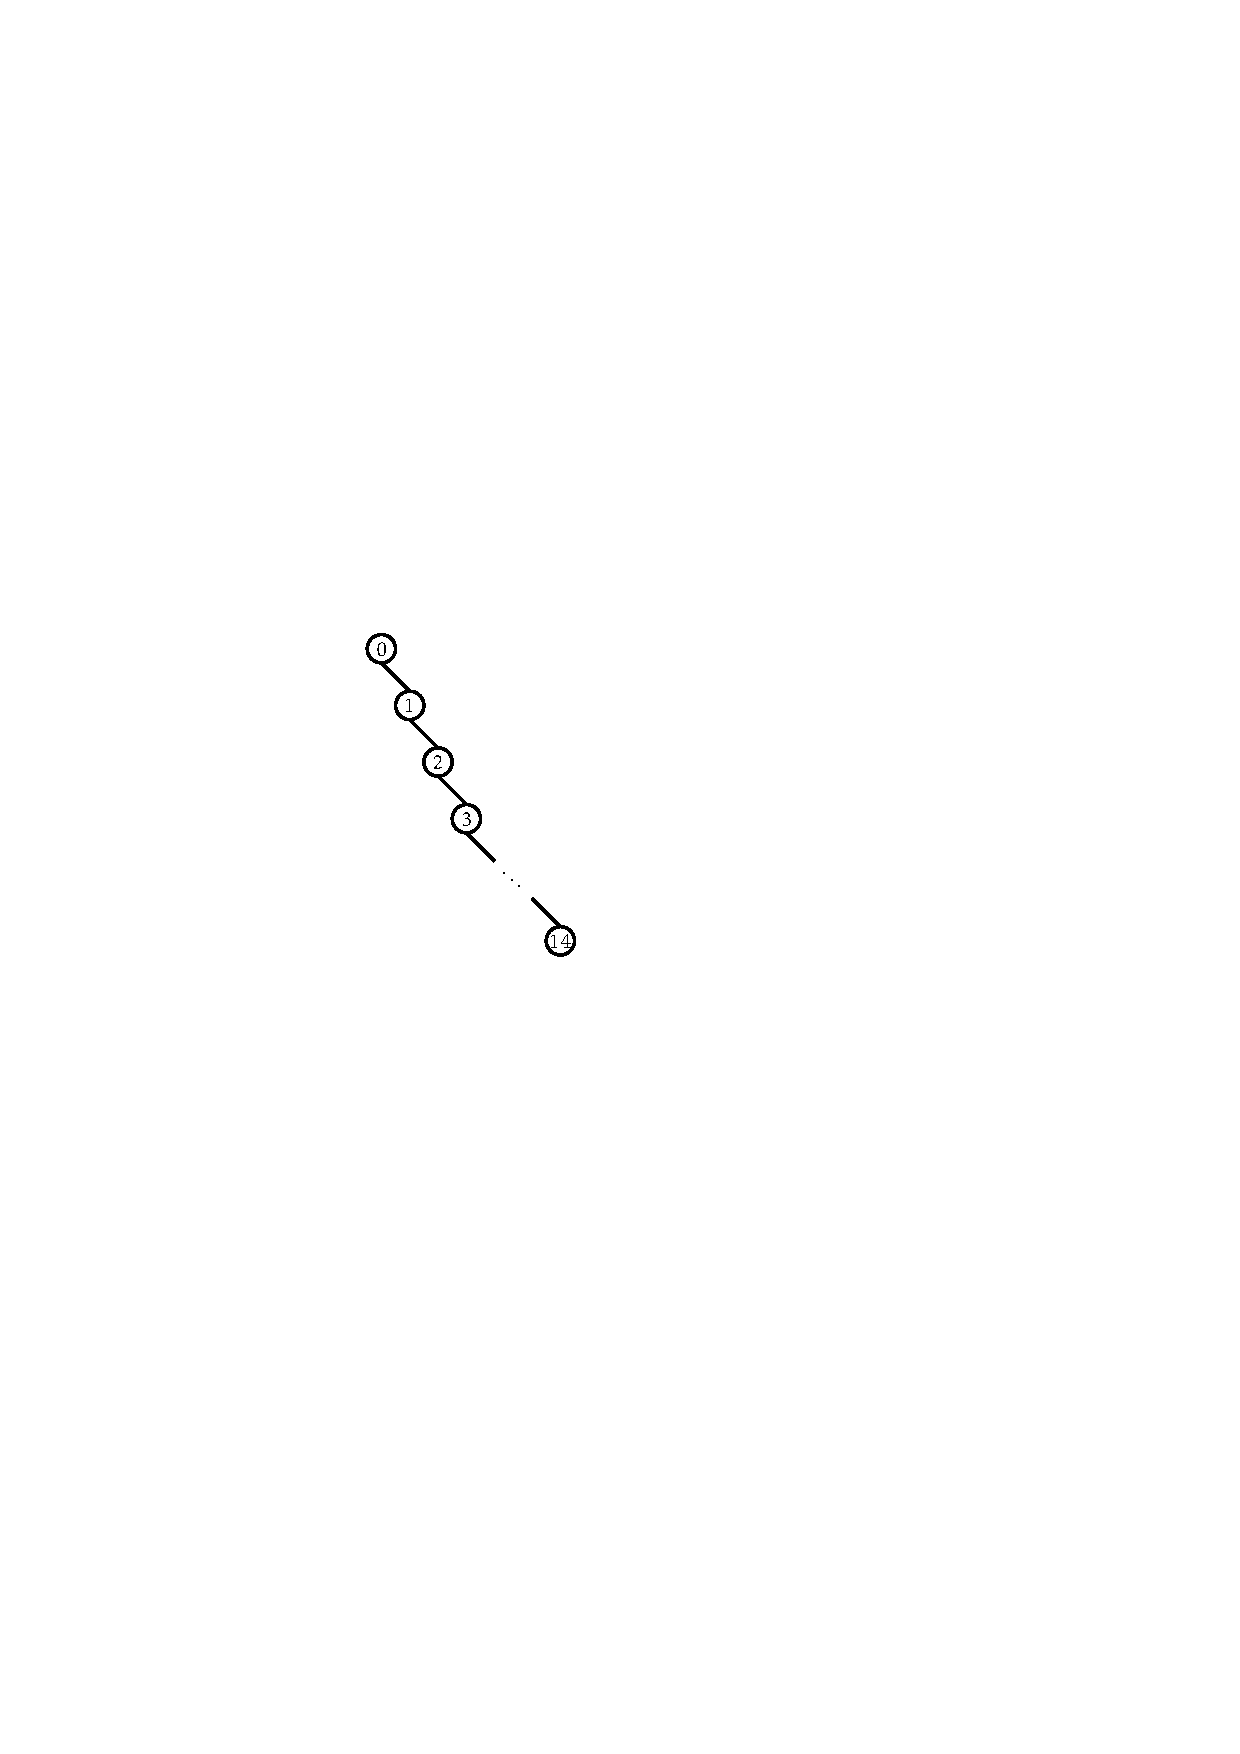
\includegraphics[scale=0.90909,scale=0.95]{figs/bst-path} &
      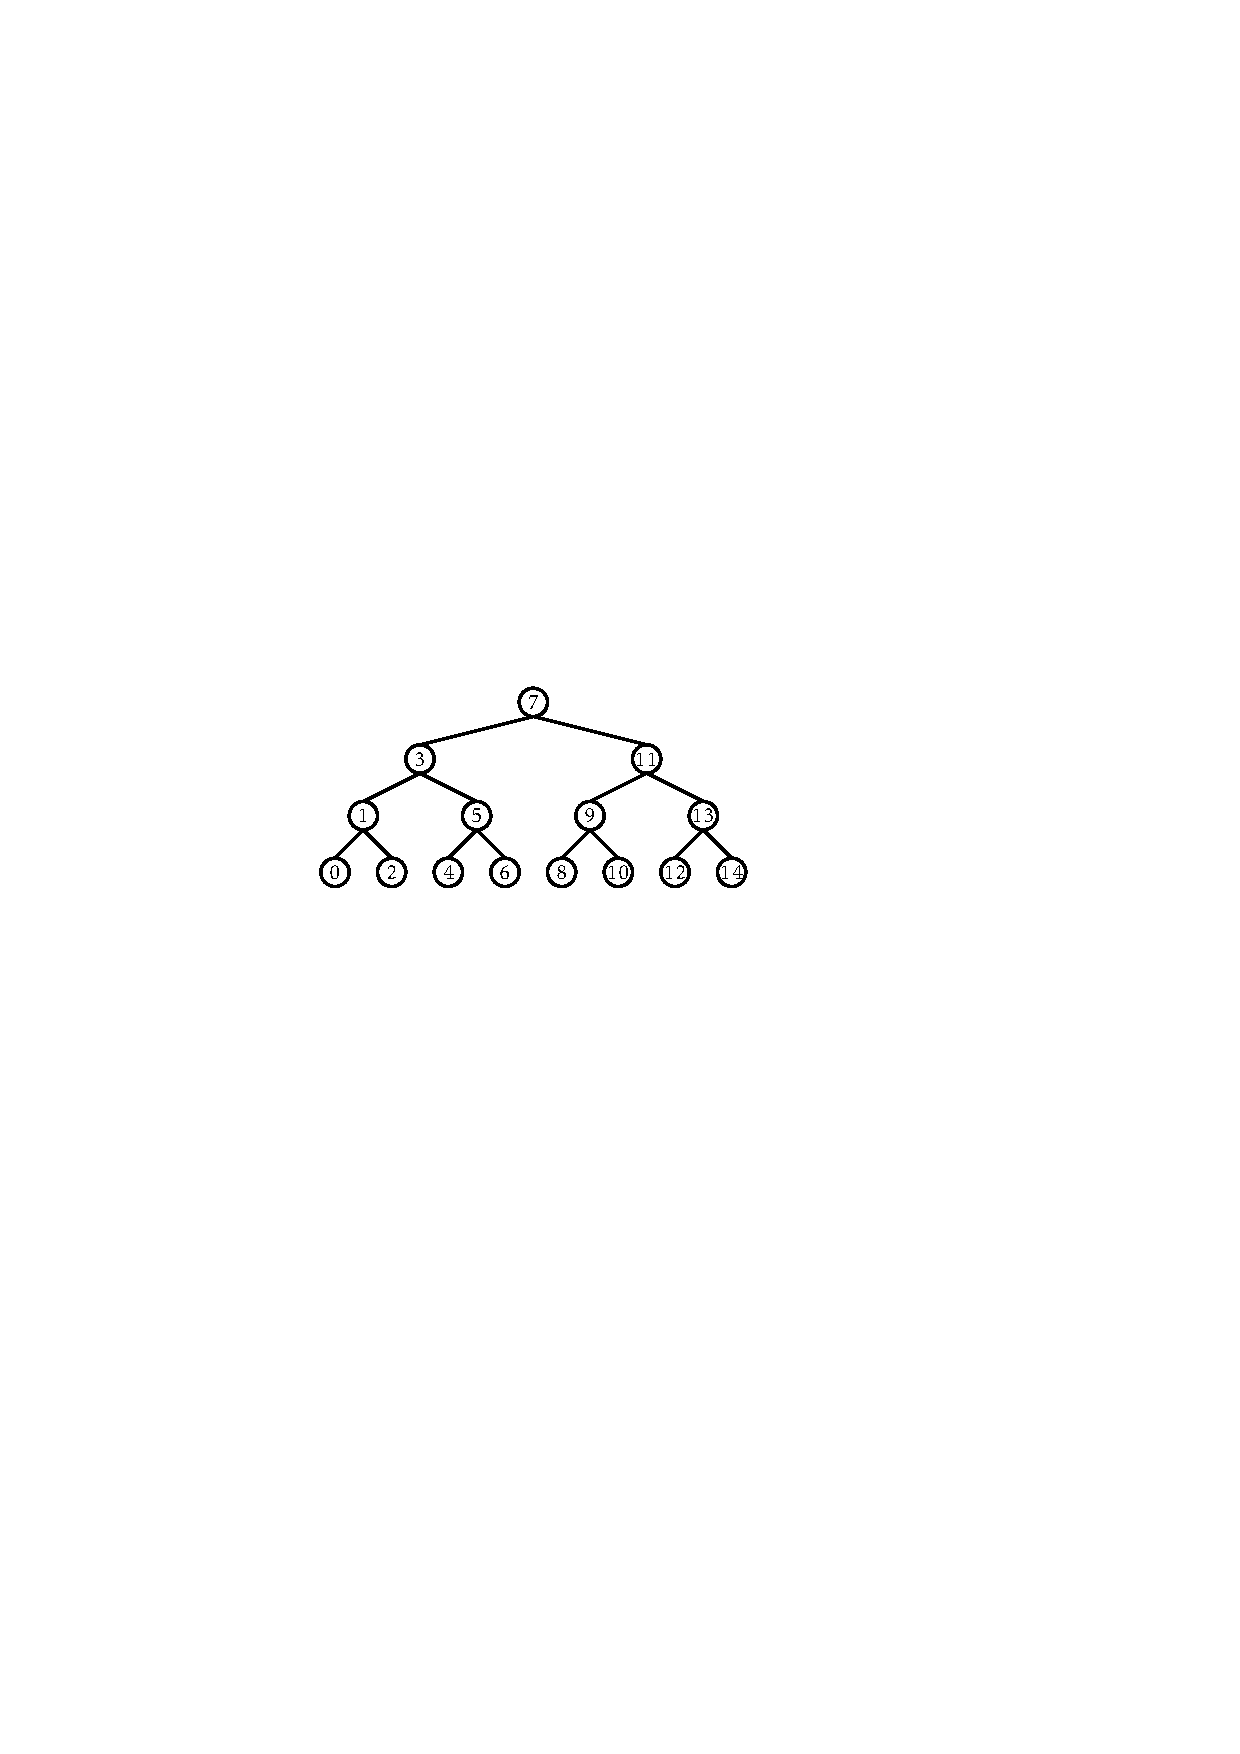
\includegraphics[scale=0.90909,scale=0.95]{figs/bst-balanced}
    \end{tabular}
  \end{center}
  \caption{Two binary search trees containing the integers $0,\ldots,14$.}
  \figlabel{rbs-lvc}
\end{figure}

Imagine how these two trees could have been constructed.  The one on
the left occurs if we start with an empty #BinarySearchTree# and add
the sequence
\[
    \langle 0,1,2,3,4,5,6,7,8,9,10,11,12,13,14 \rangle \enspace .
\]
No other sequence of additions will create this tree (as you can prove
by induction on #n#). On the other hand, the tree on the right can be
created by the sequence
\[
    \langle 7,3,11,1,5,9,13,0,2,4,6,8,10,12,14 \rangle  \enspace .
\]
Other sequences work as well, including
\[
    \langle 7,3,1,5,0,2,4,6,11,9,13,8,10,12,14 \rangle  \enspace ,
\]
and
\[
    \langle 7,3,1,11,5,0,2,4,6,9,13,8,10,12,14 \rangle \enspace .
\]
In fact, there are $21,964,800$ addition sequences that generate the
tree on the right and only one that generates the tree on the left.

The above example gives some anecdotal evidence that, if we choose a
random permutation of $0,\ldots,14$, and add it into a binary search
tree, then we are more likely to get a very balanced tree (the right
side of \figref{rbs-lvc}) than we are to get a very unbalanced tree
(the left side of \figref{rbs-lvc}).

We can formalize this notion by studying random binary search trees.
A \emph{random binary search tree}
\index{random binary search tree}%
\index{binary search tree!random}%
of size #n# is obtained in the
following way:  Take a random permutation, $#x#_0,\ldots,#x#_{#n#-1}$,
of the integers $0,\ldots,#n#-1$ and add its elements, one by one,
into a #BinarySearchTree#.  By \emph{random permutation}
\index{permutation!random}%
\index{random permutation}%
we mean that
each of the possible $#n#!$ permutations (orderings) of $0,\ldots,#n#-1$
is equally likely, so that the probability of obtaining any particular
permutation is $1/#n#!$.

Note that the values $0,\ldots,#n#-1$ could be replaced by any ordered
set of #n# elements without changing any of the properties of the
random binary search tree.  The element $#x#\in\{0,\ldots,#n#-1\}$ is
simply standing in for the element of rank #x# in an ordered set of
size #n#.

Before we can present our main result about random binary search trees,
we must take some time for a short digression to discuss a type of number
that comes up frequently when studying randomized structures. For a
non-negative integer, $k$, the $k$-th \emph{harmonic number},
\index{harmonic number}%
\index{H@$H_k$ (harmonic number)}%
denoted
$H_k$, is defined as
\[
  H_k = 1 + 1/2 + 1/3 + \cdots + 1/k \enspace .
\] 
The harmonic number $H_k$ has no simple closed form, but it is very
closely related to the natural logarithm of $k$.  In particular,
\[
  \ln k < H_k \le \ln k + 1  \enspace .
\]
\newcommand{\hint}{\int_1^k\! (1/x)\, \mathrm{d}x}%
Readers who have studied calculus might notice that this is because
the integral $\hint = \ln k$.  Keeping in mind that an integral can be
interpreted as the area between a curve and the $x$-axis, the value of
$H_k$ can be lower-bounded by the integral $\hint$ and upper-bounded by
$1+ \hint$.  (See \figref{harmonic-integral} for a graphical explanation.)

\begin{figure}
  \begin{center}
    \begin{tabular}{cc}
      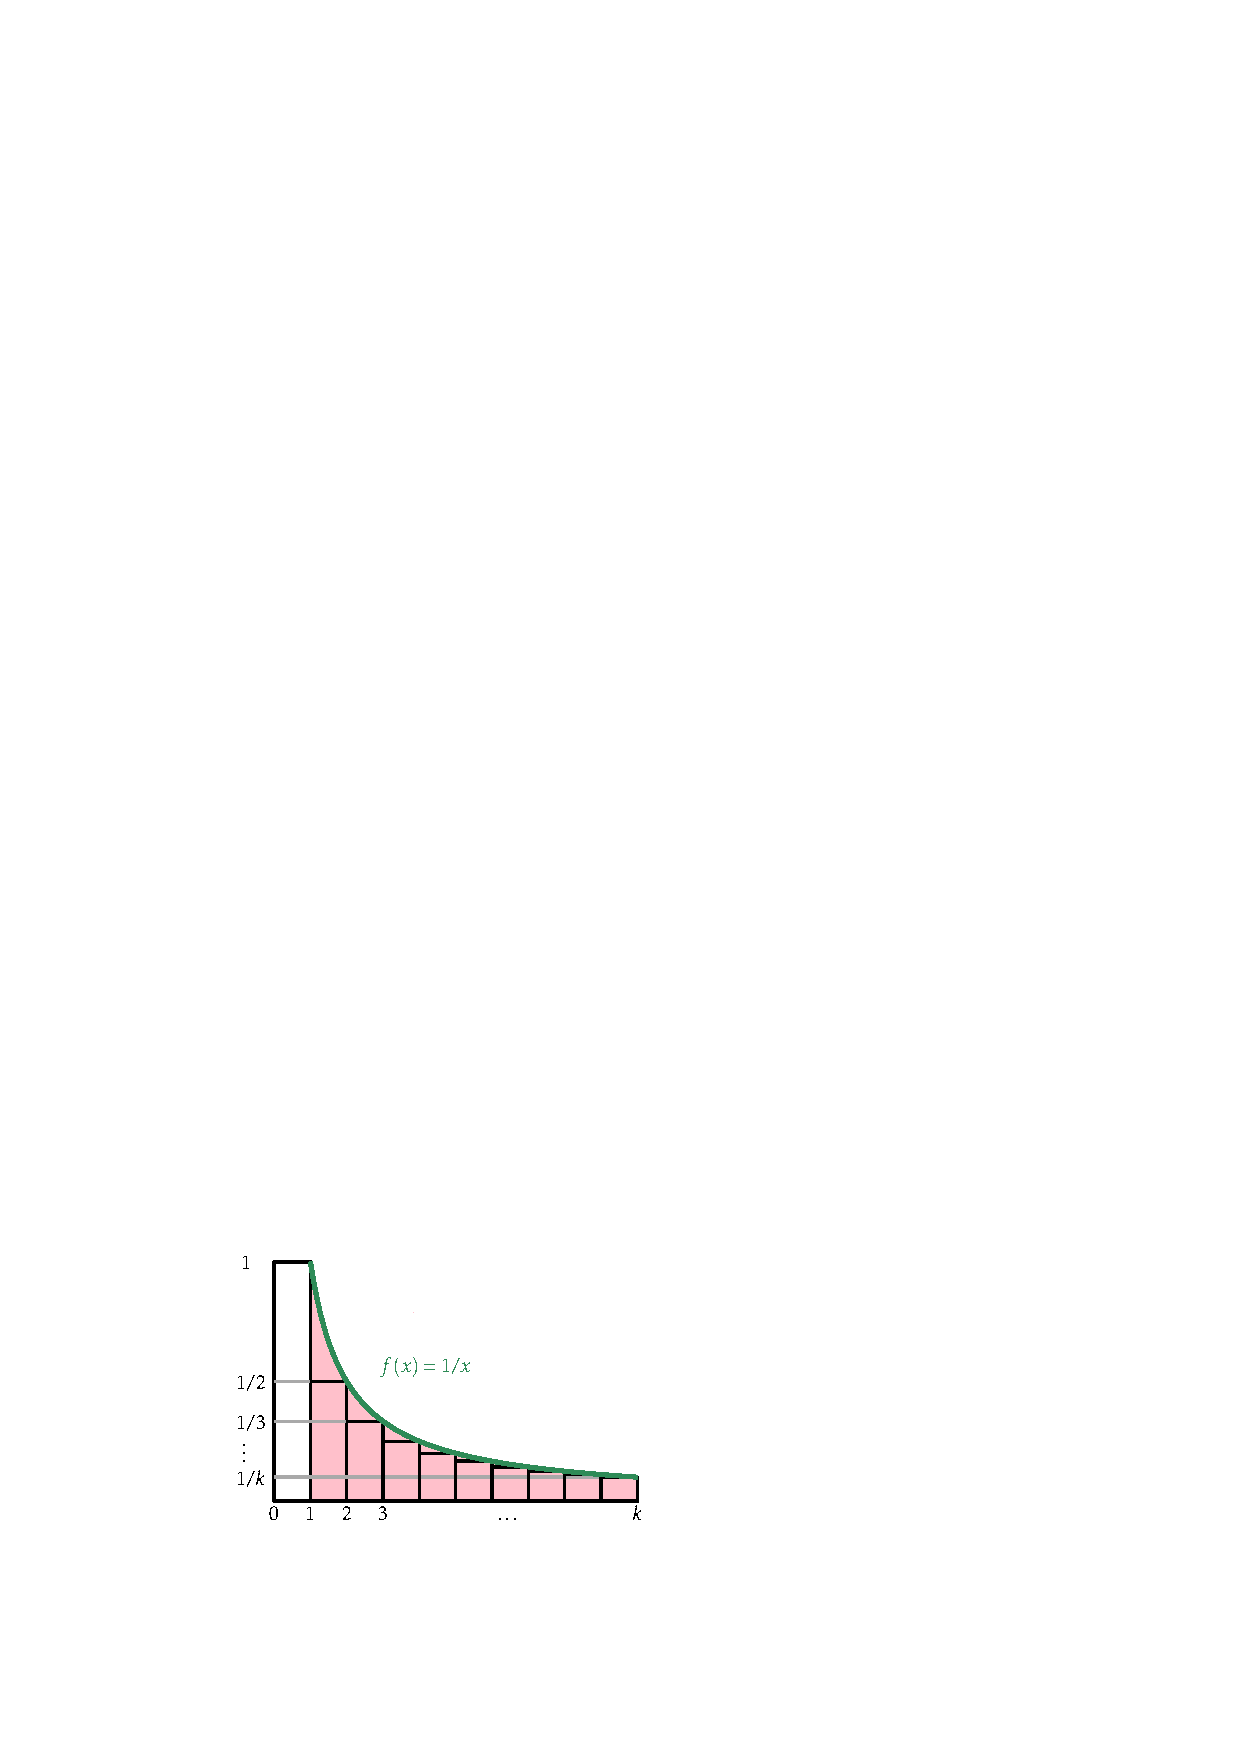
\includegraphics[width=\HalfScaleIfNeeded]{figs/harmonic-2} 
        & 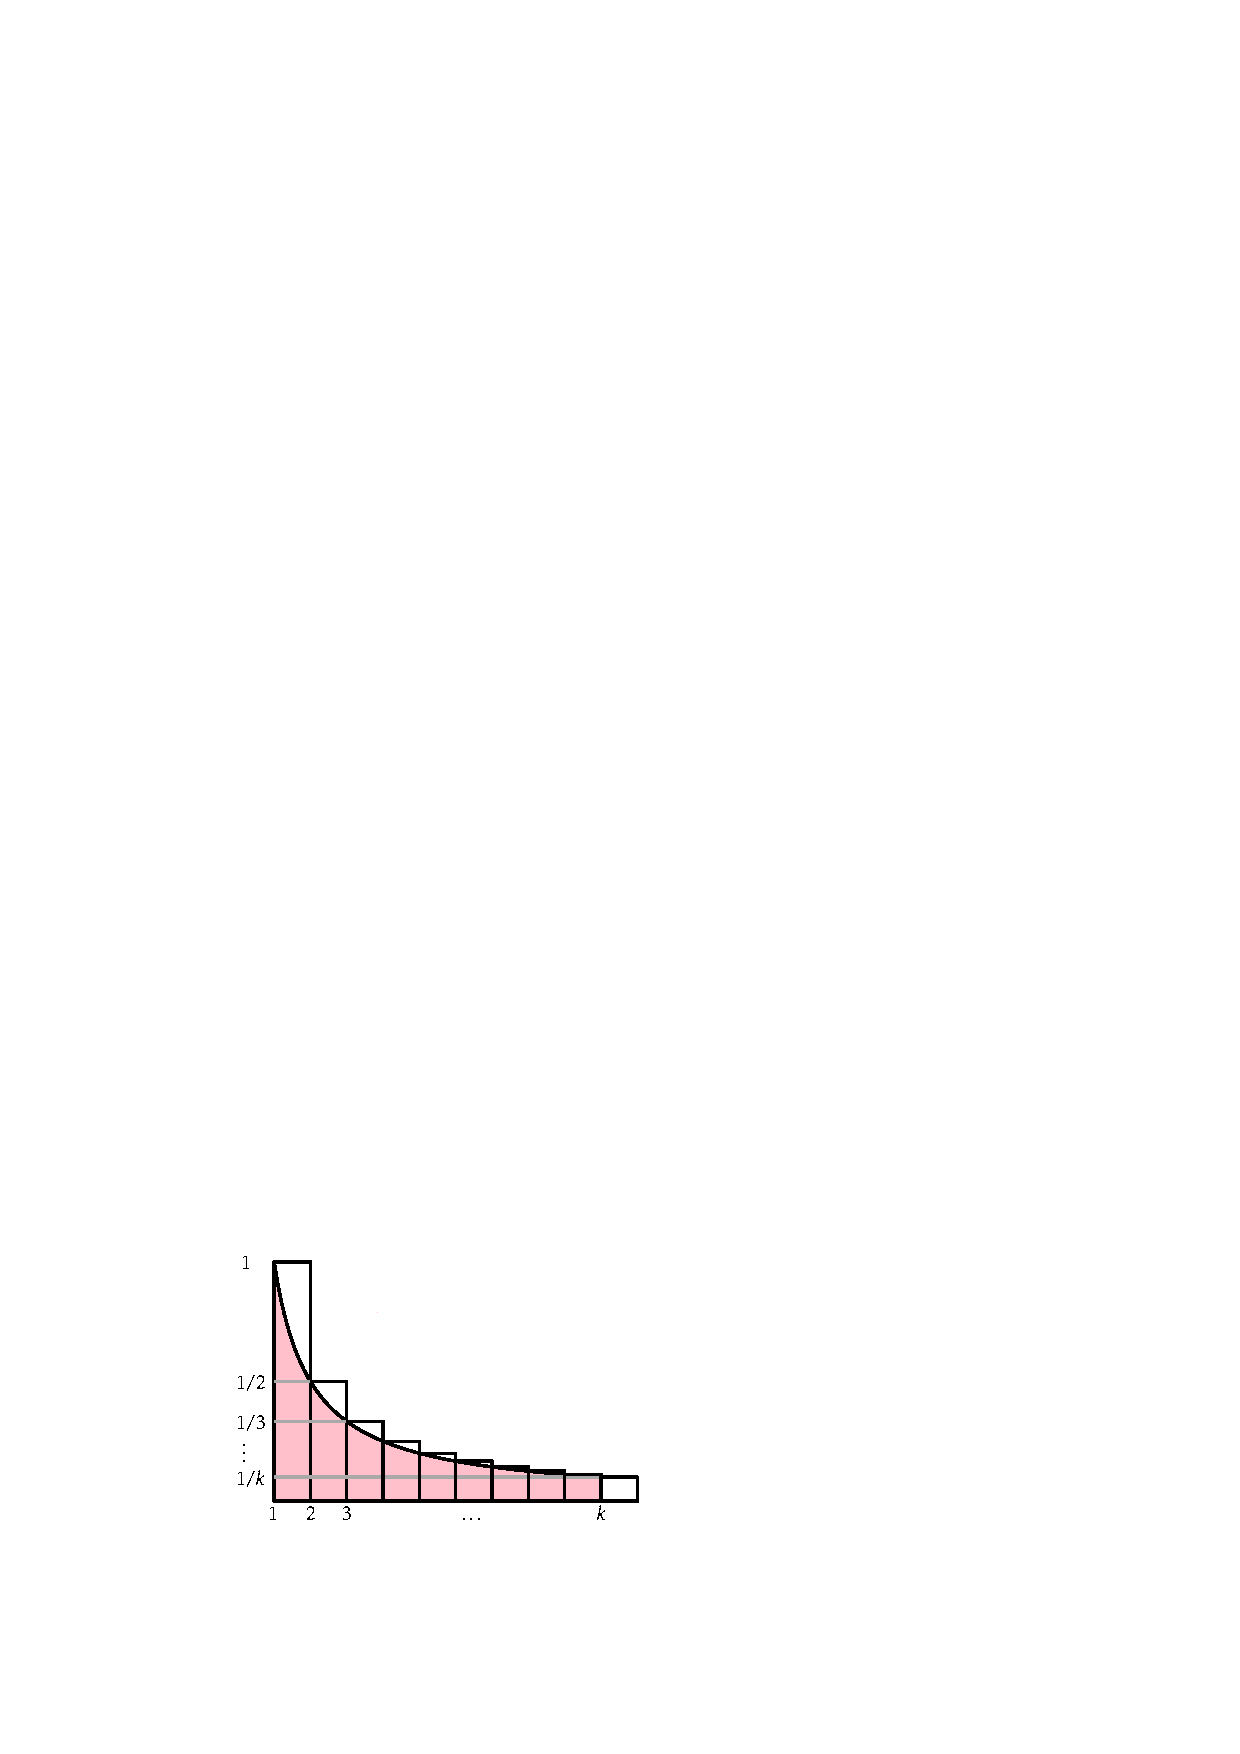
\includegraphics[width=\HalfScaleIfNeeded]{figs/harmonic-3}
    \end{tabular}
  \end{center}
  \caption{The $k$th harmonic number $H_k=\sum_{i=1}^k 1/i$ is upper- and lower-bounded by two integrals. The value of these integrals is given by the 
  area of the shaded region, while the value of $H_k$ is given by the area of
  the rectangles.}
  \figlabel{harmonic-integral}
\end{figure}


\begin{lem}\lemlabel{rbs}
  In a random binary search tree of size #n#, the following statements hold:
  \begin{enumerate}
    \item For any $#x#\in\{0,\ldots,#n#-1\}$, the expected length of the
    search path for #x# is $H_{#x#+1} + H_{#n#-#x#} - O(1)$.\footnote{The
    expressions $#x#+1$ and $#n#-#x#$ can be interpreted respectively
    as the number of elements in the tree less than or equal to #x#
    and the number of elements in the tree greater than or equal to #x#.}
    \item For any $#x#\in(-1,n)\setminus\{0,\ldots,#n#-1\}$, the
    expected length of the search path for #x# is $H_{\lceil#x#\rceil}
    + H_{#n#-\lceil#x#\rceil}$.
  \end{enumerate}
\end{lem}

We will prove \lemref{rbs} in the next section.  For now, consider what
the two parts of \lemref{rbs} tell us.  The first part tells us that if
we search for an element in a tree of size #n#, then the expected length
of the search path is at most $2\ln n + O(1)$.  The second part tells
us the same thing about searching for a value not stored in the tree.
When we compare the two parts of the lemma, we see that it is only
slightly faster to search for something that is in the tree compared to
something that is not.


\subsection{Proof of \lemref{rbs}}

The key observation needed to prove \lemref{rbs} is the following:
The search path for a value #x# in the open interval $(-1,#n#)$ in a
random binary search tree, $T$, contains the node with key $i < #x#$
if, and only if, in the random permutation used to create $T$, $i$
appears before any of $\{i+1,i+2,\ldots,\lfloor#x#\rfloor\}$.

To see this, refer to \figref{rbst-records} and notice that until
some value in $\{i,i+1,\ldots,\lfloor#x#\rfloor\}$ is added, the search
paths for each value in the open interval $(i-1,\lfloor#x#\rfloor+1)$
are identical.  (Remember that for two values to have
different search paths, there must be some element in the tree that
compares differently with them.)  Let $j$ be the first element in
$\{i,i+1,\ldots,\lfloor#x#\rfloor\}$ to appear in the random permutation.
Notice that $j$ is now and will always be on the search path for #x#.
If $j\neq i$ then the node $#u#_j$ containing $j$ is created before the
node $#u#_i$ that contains $i$.  Later, when $i$ is added, it will be
added to the subtree rooted at $#u#_j#.left#$, since $i<j$.  On the other
hand, the search path for #x# will never visit this subtree because it
will proceed to $#u#_j#.right#$ after visiting $#u#_j$.

\begin{figure}
  \begin{center}
    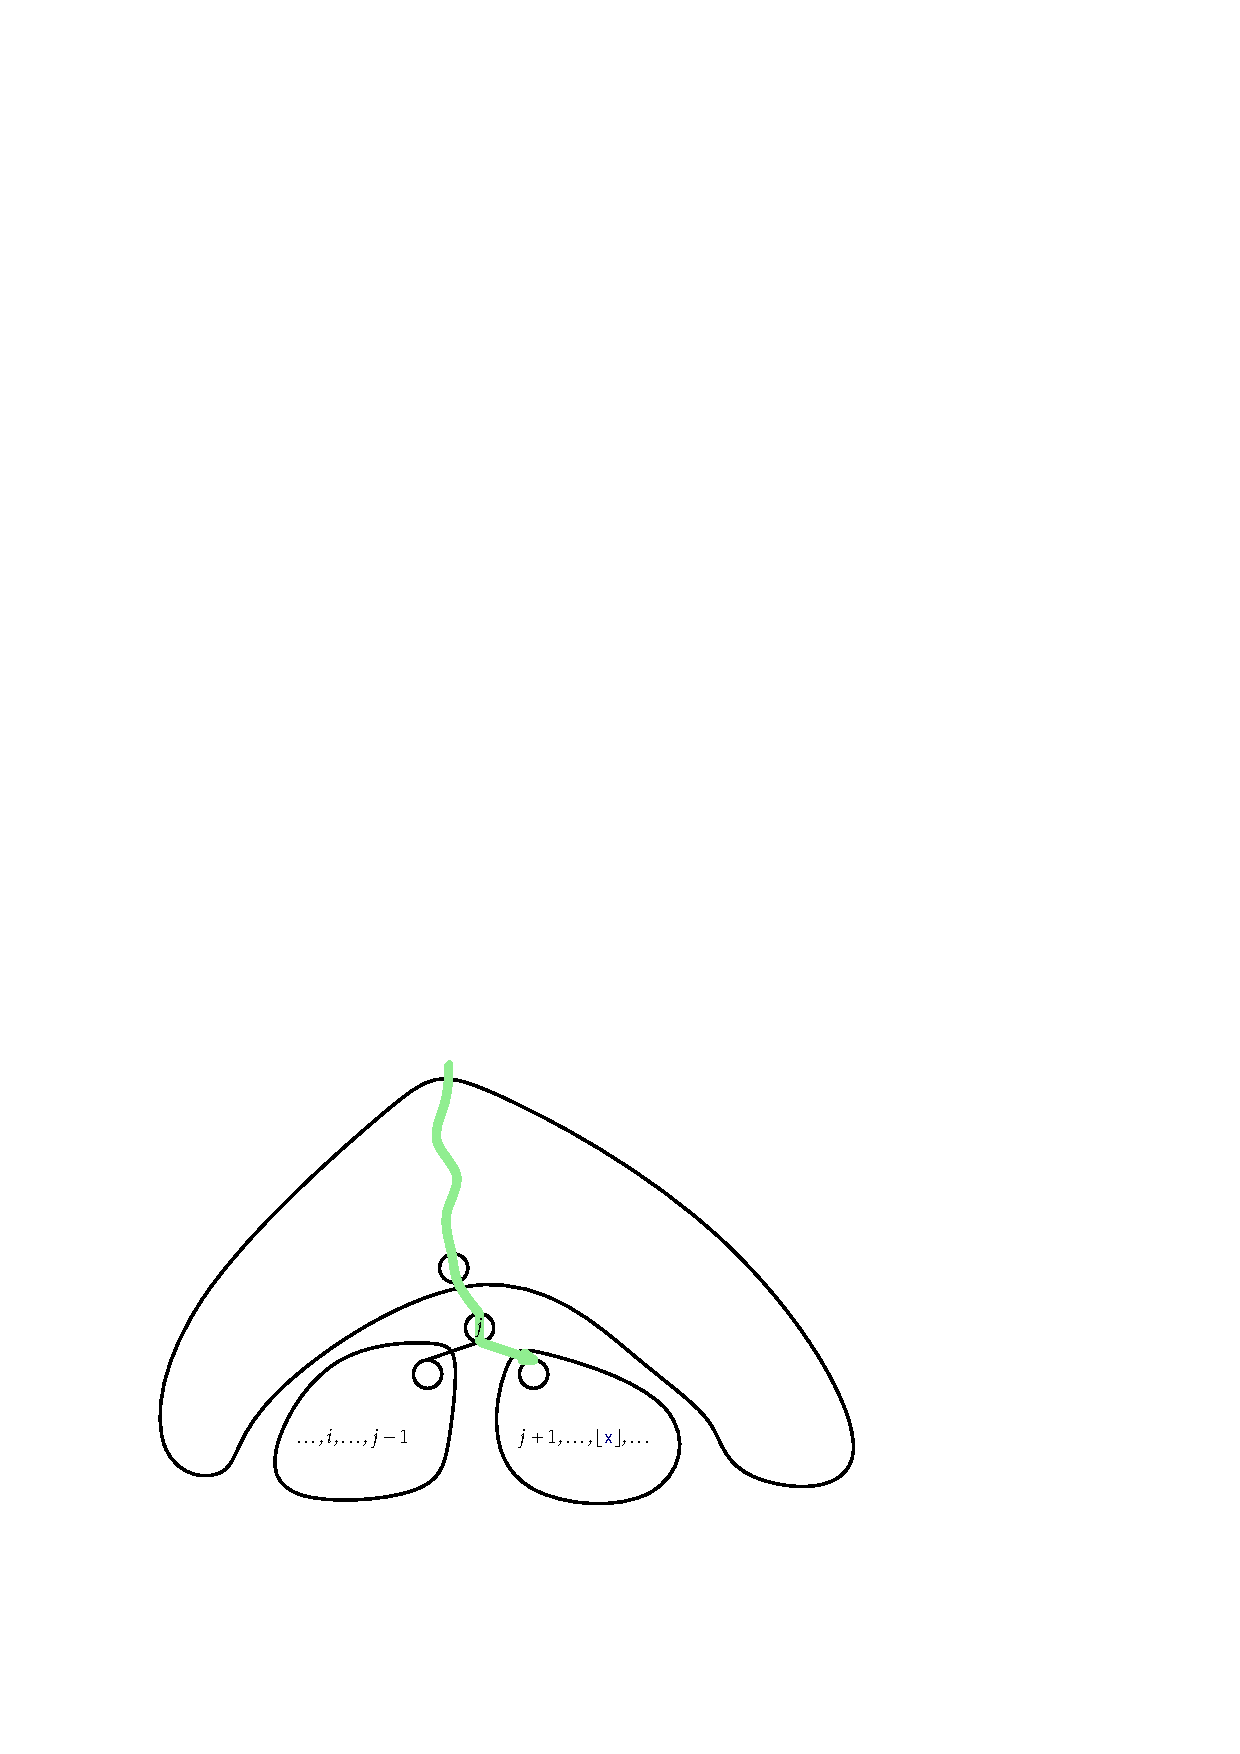
\includegraphics[width=\ScaleIfNeeded]{figs/rbst-records}
  \end{center}
  \caption[The search path in a random binary search tree]{The value $i<#x#$ is on the search path for #x# if and only
   if $i$ is the first element among $\{i,i+1,\ldots,\lfloor#x#\rfloor\}$ added to the tree.}
  \figlabel{rbst-records}
\end{figure}

Similarly, for $i>#x#$, $i$ appears in the search path for #x#
if and only if $i$ appears before any of $\{\lceil#x#\rceil,
\lceil#x#\rceil+1,\ldots,i-1\}$ in the random permutation used to
create $T$.

Notice that, if we start with a random permutation of $\{0,\ldots,#n#\}$,
then the subsequences containing only $\{i,i+1,\ldots,\lfloor#x#\rfloor\}$
and $\{\lceil#x#\rceil, \lceil#x#\rceil+1,\ldots,i-1\}$ are also random
permutations of their respective elements.  Each element, then, in the
subsets $\{i,i+1,\ldots,\lfloor#x#\rfloor\}$ and $\{\lceil#x#\rceil,
\lceil#x#\rceil+1,\ldots,i-1\}$ is equally likely to appear before
any other in its subset in the random permutation used to create $T$.
So we have
\[
  \Pr\{\mbox{$i$ is on the search path for #x#}\}
  = \left\{ \begin{array}{ll}
     1/(\lfloor#x#\rfloor-i+1) & \mbox{if $i < #x#$} \\
     1/(i-\lceil#x#\rceil+1) & \mbox{if $i > #x#$} 
     \end{array}\right . \enspace .
\]

With this observation, the proof of \lemref{rbs}
involves some simple calculations with harmonic numbers:

\begin{proof}[Proof of \lemref{rbs}]
Let $I_i$ be the indicator random variable that is equal to one when $i$
appears on the search path for #x# and zero otherwise.  Then the length
of the search path is given by
\[
  \sum_{i\in\{0,\ldots,#n#-1\}\setminus\{#x#\}} I_i
\]
so, if $#x#\in\{0,\ldots,#n#-1\}$, the expected length of the search
path is given by (see \figref{rbst-probs}.a)
\begin{align*}
  \E\left[\sum_{i=0}^{#x#-1} I_i + \sum_{i=#x#+1}^{#n#-1} I_i\right]
   & =  \sum_{i=0}^{#x#-1} \E\left[I_i\right]
         + \sum_{i=#x#+1}^{#n#-1} \E\left[I_i\right] \\
   & = \sum_{i=0}^{#x#-1} 1/(\lfloor#x#\rfloor-i+1)
         + \sum_{i=#x#+1}^{#n#-1} 1/(i-\lceil#x#\rceil+1) \\
   & = \sum_{i=0}^{#x#-1} 1/(#x#-i+1)
         + \sum_{i=#x#+1}^{#n#-1} 1/(i-#x#+1) \\
   & = \frac{1}{2}+\frac{1}{3}+\cdots+\frac{1}{#x#+1} \\
   & \quad {} + \frac{1}{2}+\frac{1}{3}+\cdots+\frac{1}{#n#-#x#} \\
   & = H_{#x#+1} + H_{#n#-#x#} - 2  \enspace .
\end{align*}
The corresponding calculations for a search value
$#x#\in(-1,n)\setminus\{0,\ldots,#n#-1\}$ are almost identical (see
\figref{rbst-probs}.b).
\end{proof}

\begin{figure}
  \begin{center}
    \begin{tabular}{@{}c@{}}
      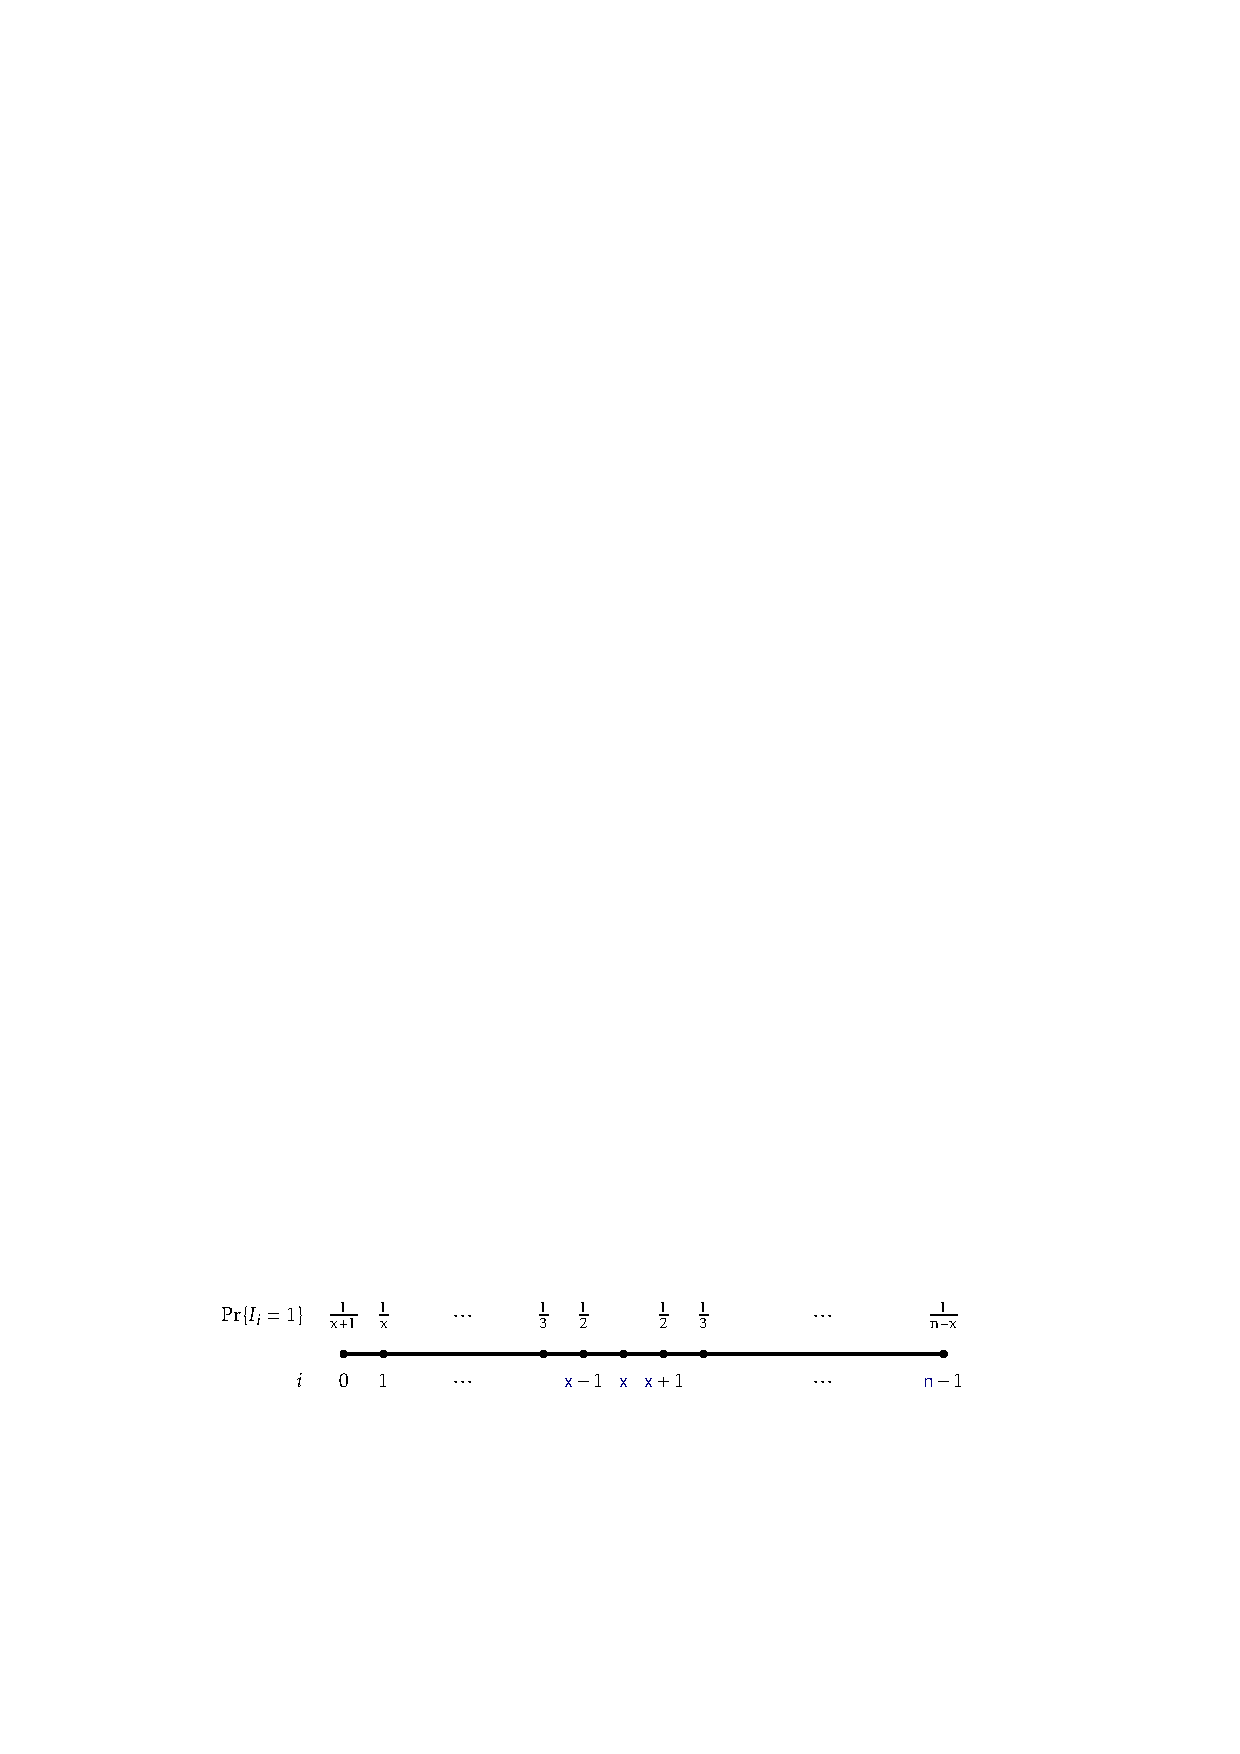
\includegraphics[width=\ScaleIfNeeded]{figs/rbst-probs-a} \\ (a) \\[2ex]
      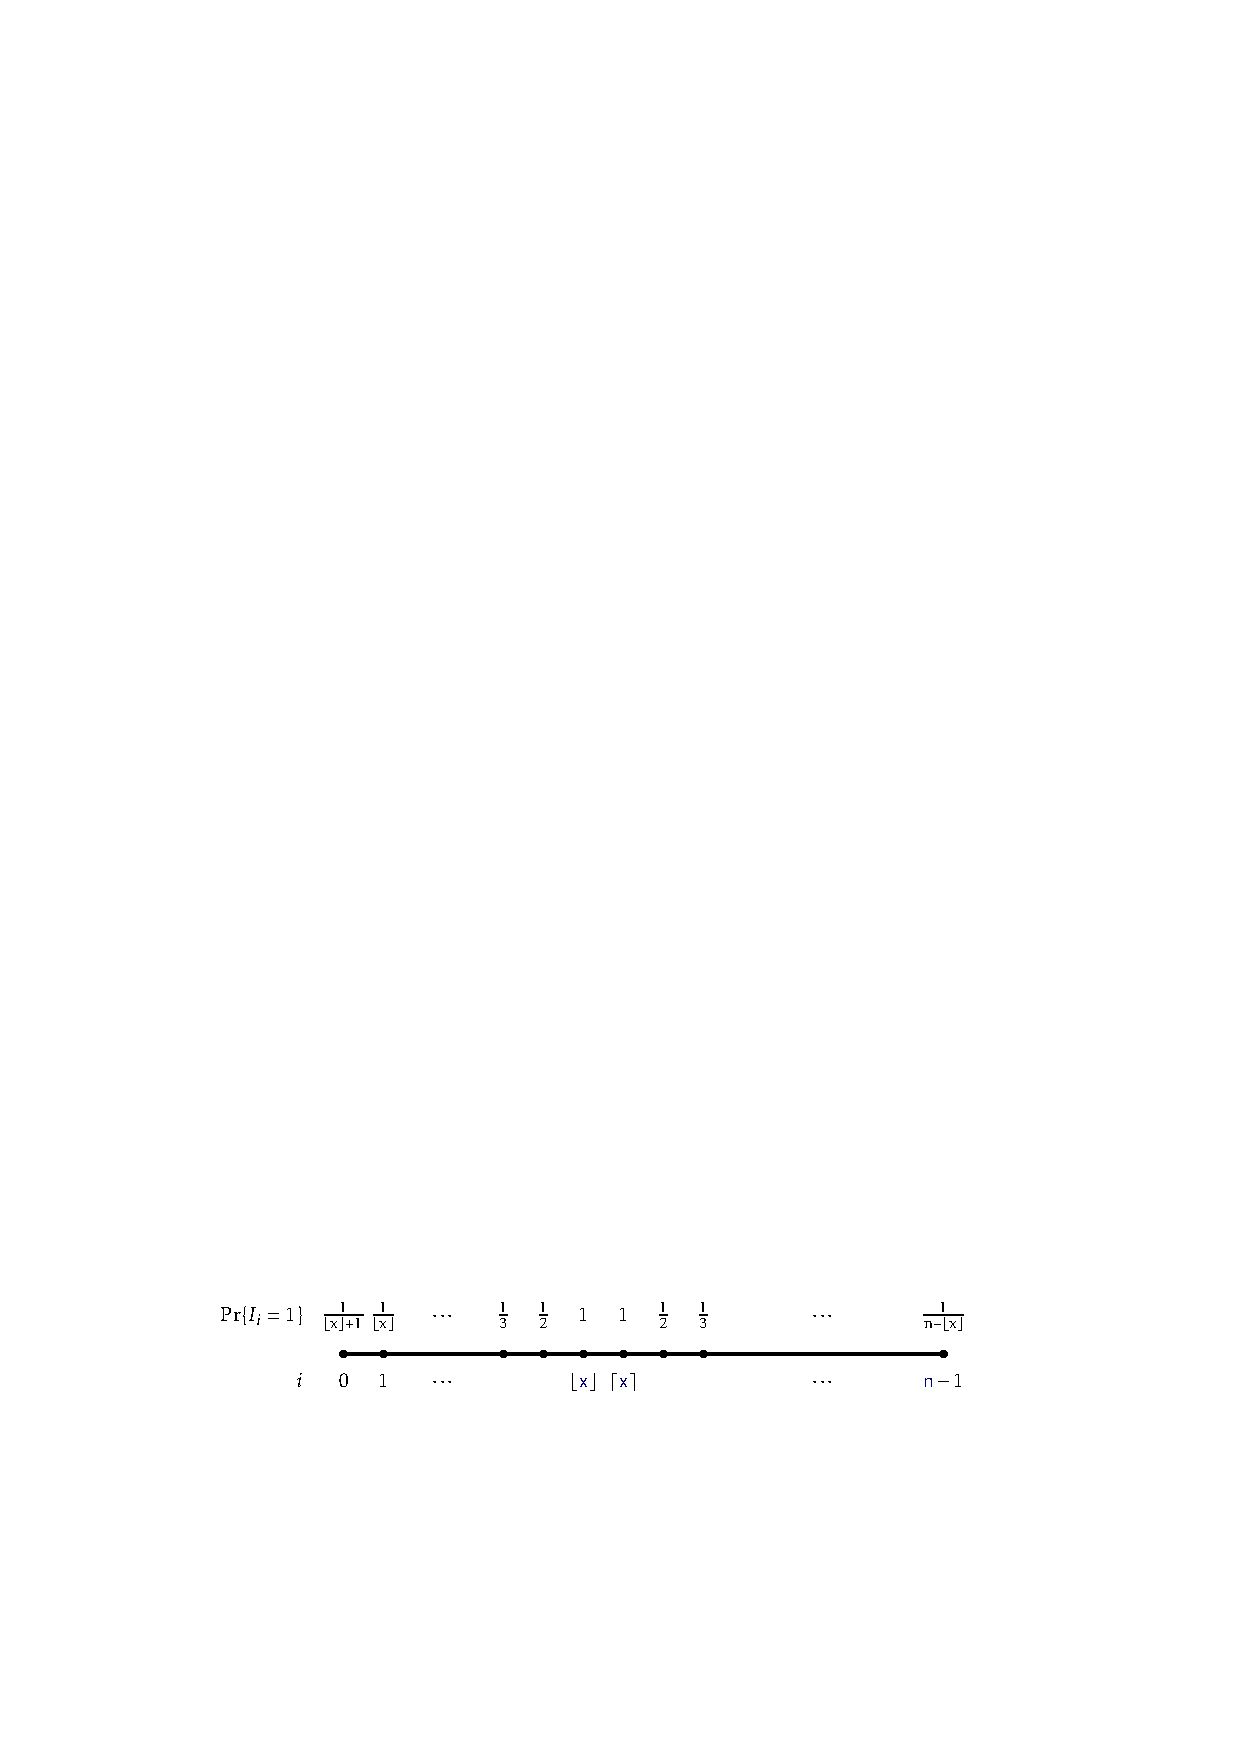
\includegraphics[width=\ScaleIfNeeded]{figs/rbst-probs-b} \\ (b) \\[2ex]
    \end{tabular}
  \end{center}
  \caption[The probabilities of an element being on a search path]{The probabilities of an element being on the search path for #x#
   when (a)~#x# is an integer and (b)~when #x# is not an integer.}
  \figlabel{rbst-probs}
\end{figure}

\subsection{Summary}

The following theorem summarizes the performance of a random binary
search tree:

\begin{thm}\thmlabel{rbs}
A random binary search tree can be constructed in $O(#n#\log #n#)$ time.
In a random binary search tree, the #find(x)# operation takes $O(\log
#n#)$ expected time.
\end{thm}

We should emphasize again that the expectation in \thmref{rbs} is with
respect to the random permutation used to create the random binary
search tree.  In particular, it does not depend on a random choice of
#x#; it is true for every value of #x#.


\section{#Treap#: A Randomized Binary Search Tree}
\seclabel{treap}

\index{Treap@#Treap#}%
The problem with random binary search trees is, of course, that they are
not dynamic.  They don't support the #add(x)# or #remove(x)# operations
needed to implement the #SSet# interface.  In this section we describe
a data structure called a #Treap# that uses \lemref{rbs} to implement
the #SSet# interface.\footnote{The name #Treap# comes from the fact
that this data structure is simultaneously a binary search \textbf{tr}ee
(\secref{binarysearchtree}) and a h\textbf{eap} (\chapref{heaps}).}

A node in a #Treap# is like a node in a #BinarySearchTree# in that it has
a data value, #x#, but it also contains a unique numerical \emph{priority},
#p#, that is assigned at random:
\javaimport{ods/Treap.Node<T>}
\cppimport{ods/Treap.TreapNode}
In addition to being a binary search tree, the nodes in a #Treap#
also obey the \emph{heap property}:
\begin{itemize}
\item (Heap Property)  At every node #u#, except the root, 
      $#u.parent.p# < #u.p#$.
      \index{heap property}%
\end{itemize}
In other words, each node has a priority smaller than that of its two
children.  An example is shown in \figref{treap}.

\begin{figure}
  \begin{center}
    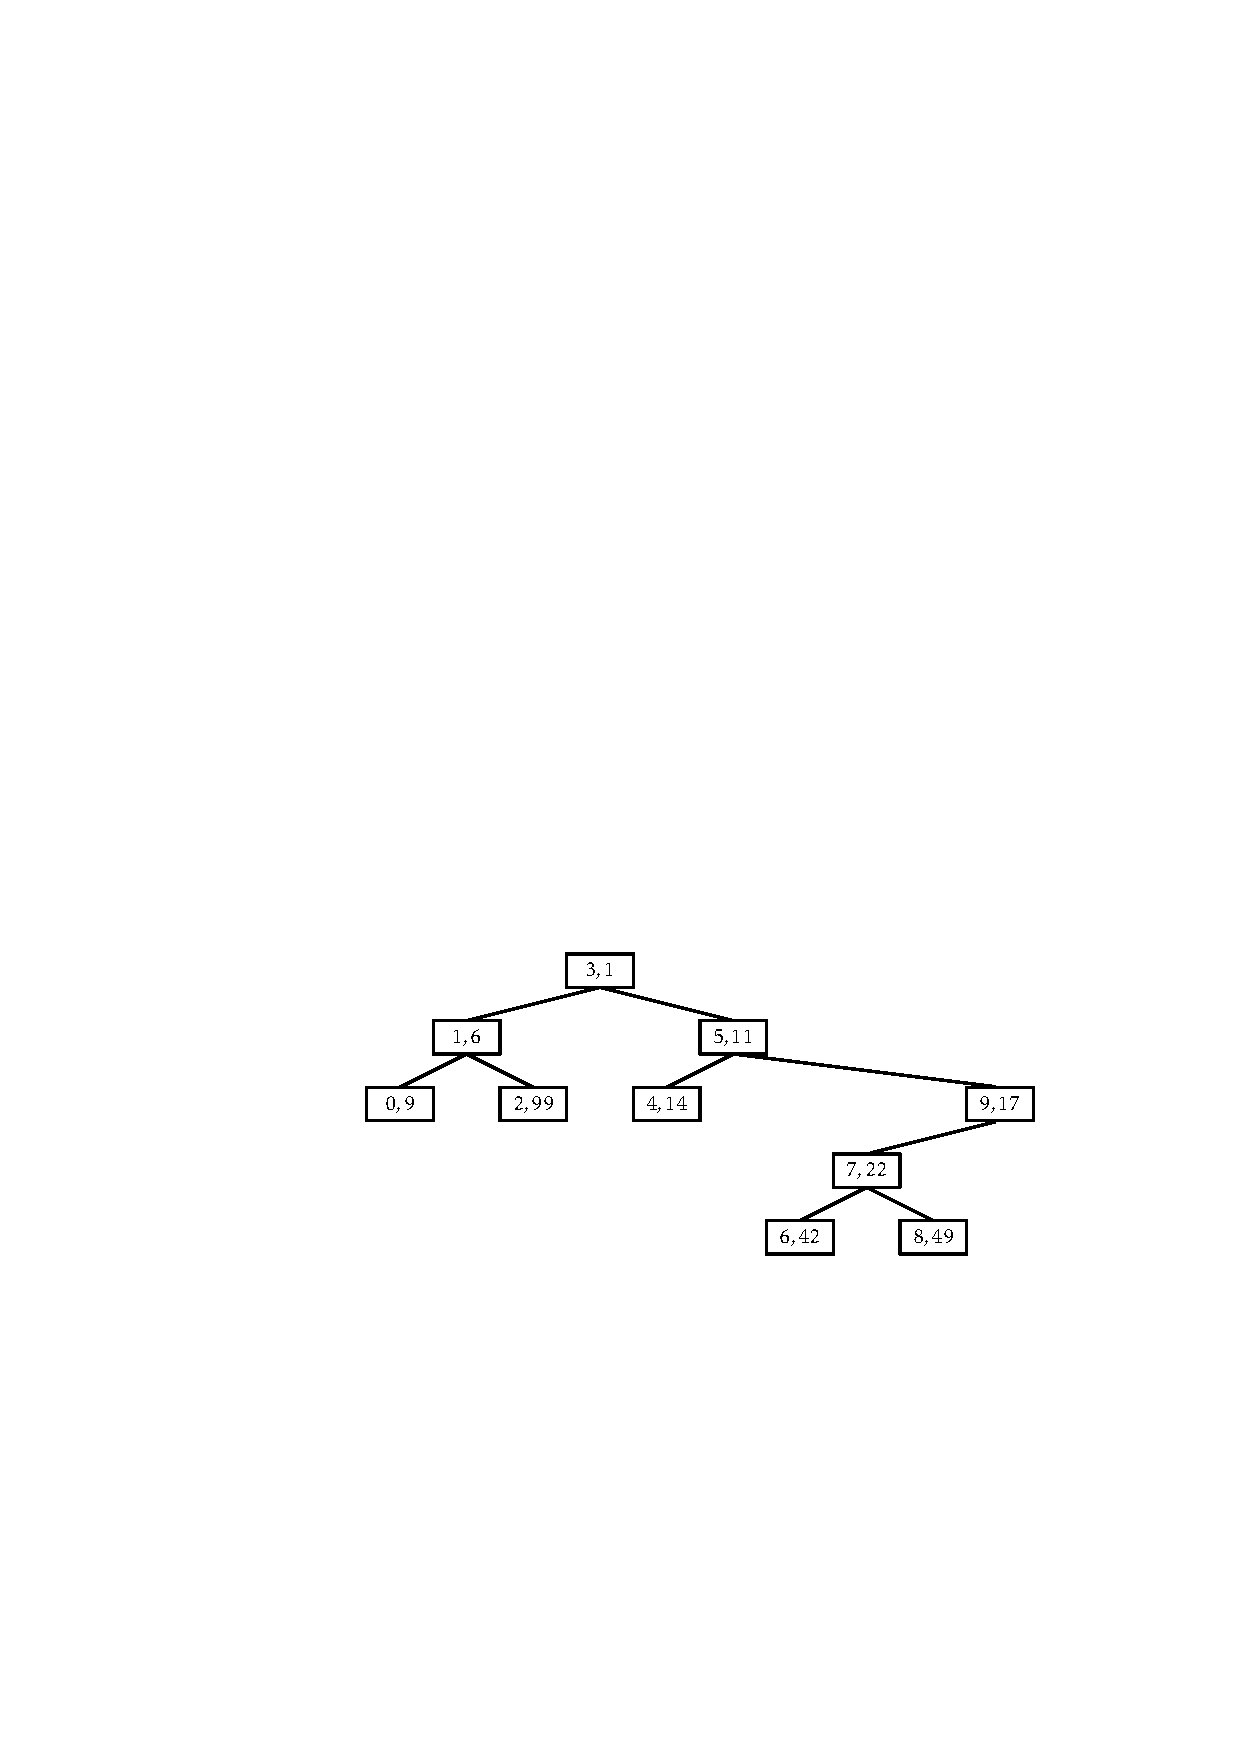
\includegraphics[width=\ScaleIfNeeded]{figs/treap}
  \end{center}
  \caption[A Treap]{An example of a #Treap# containing the integers
  $0,\ldots,9$. Each node, #u#, is illustrated as a box containing $#u.x#,#u.p#$.}
  \figlabel{treap}
\end{figure}

The heap and binary search tree conditions together ensure that, once
the key (#x#) and priority (#p#) for each node are defined, the
shape of the #Treap# is completely determined. The heap property tells us that
the node with minimum priority has to be the root, #r#, of the #Treap#.
The binary search tree property tells us that all nodes with keys smaller
than #r.x# are stored in the subtree rooted at #r.left# and all nodes
with keys larger than #r.x# are stored in the subtree rooted at #r.right#.

The important point about the priority values in a #Treap# is that they
are unique and assigned at random.  Because of this, there are
two equivalent ways we can think about a #Treap#.  As defined above, a
#Treap# obeys the heap and binary search tree properties.  Alternatively,
we can think of a #Treap# as a #BinarySearchTree# whose nodes
were added in increasing order of priority.  For example, the #Treap#
in \figref{treap} can be obtained by adding the sequence of $(#x#,#p#)$
values 
\[
  \langle
   (3,1), (1,6), (0,9), (5,11), (4,14), (9,17), (7,22), (6,42), (8,49), (2,99)
  \rangle
\]
into a #BinarySearchTree#.

Since the priorities are chosen randomly, this is equivalent to taking a
random permutation of the keys---in this case the permutation is
\[
  \langle 3, 1, 0, 5, 9, 4, 7, 6, 8, 2 \rangle
\]
---and adding these to a #BinarySearchTree#.  But this means that the
shape of a treap is identical to that of a random binary search tree.
In particular, if we replace each key #x# by its rank,\footnote{The
rank of an element #x# in a set $S$ of elements is the number of
elements in $S$ that are less than #x#.} then \lemref{rbs} applies.
Restating \lemref{rbs} in terms of #Treap#s, we have:
\begin{lem}\lemlabel{rbs-treap}
  In a #Treap# that stores a set $S$ of #n# keys, the following statements hold:
  \begin{enumerate}
    \item For any $#x#\in S$, the expected length of
    the search path for #x# is $H_{r(#x#)+1} + H_{#n#-r(#x#)} - O(1)$.
    \item For any $#x#\not\in S$, the expected length of the
    search path for #x# is $H_{r(#x#)} + H_{#n#-r(#x#)}$.
  \end{enumerate}
  Here, $r(#x#)$ denotes the rank of #x# in the set $S\cup\{#x#\}$.
\end{lem}
Again, we emphasize that the expectation in \lemref{rbs-treap} is taken
over the random choices of the priorities for each node.  It does not
require any assumptions about the randomness in the keys.

\lemref{rbs-treap} tells us that #Treap#s can implement the #find(x)#
operation efficiently. However, the real benefit of a #Treap# is that
it can support the #add(x)# and #delete(x)# operations.  To
do this, it needs to perform rotations in order to maintain the heap property.  Refer to \figref{rotations}.
A \emph{rotation}
\index{rotation}%
in a binary
search tree is a local modification that takes a parent #u# of a node #w#
and makes #w# the parent of #u#, while preserving the binary search tree
property. Rotations come in two flavours: \emph{left} or \emph{right}
depending on whether #w# is a right or left child of #u#, respectively.
\index{left rotation}%
\index{right rotation}%

\begin{figure}
  \begin{center}
     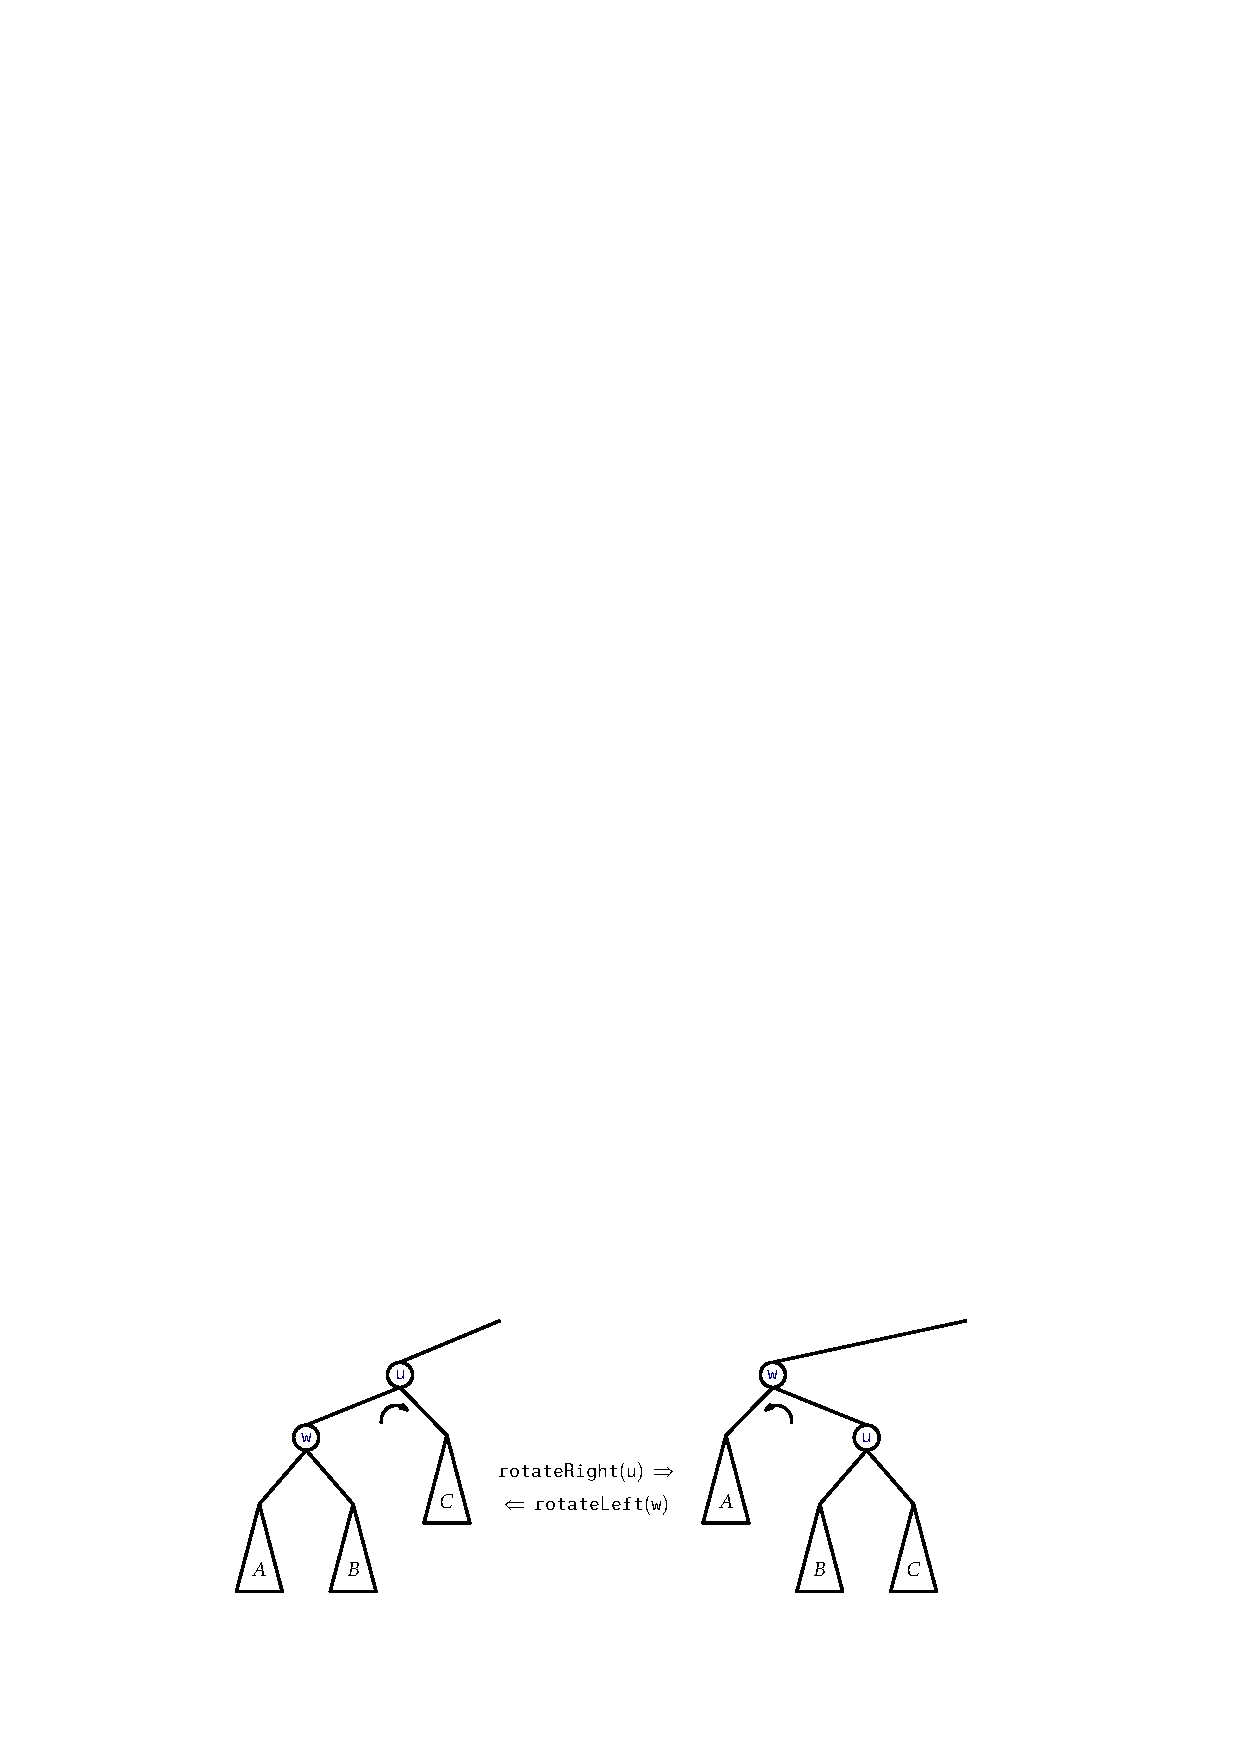
\includegraphics[width=\ScaleIfNeeded]{figs/rotation}
  \end{center}
  \caption{Left and right rotations in a binary search tree.}
  \figlabel{rotations}
\end{figure}

The code that implements this has to handle these two possibilities and
be careful of a boundary case (when #u# is the root), so the actual code
is a little longer than \figref{rotations} would lead a reader to believe:
\codeimport{ods/BinarySearchTree.rotateLeft(u).rotateRight(u)}
\label{page:rotations}
In terms of the #Treap# data structure, the most important property of a
rotation is that the depth of #w# decreases by one while the depth of #u#
increases by one.

Using rotations, we can implement the #add(x)# operation as follows:
We create a new node, #u#, assign #u.x=x#, and pick a random value
for #u.p#.  Next we add #u# using the usual #add(x)# algorithm
for a #BinarySearchTree#, so that #u# is now a leaf of the #Treap#.
At this point, our #Treap# satisfies the binary search tree property,
but not necessarily the heap property.  In particular, it may be the
case that #u.parent.p > u.p#.  If this is the case, then we perform a
rotation at node #w#=#u.parent# so that #u# becomes the parent of #w#.
If #u# continues to violate the heap property, we will have to repeat this, decreasing #u#'s depth by one every time, until
#u# either becomes the root or $#u.parent.p# < #u.p#$.
\codeimport{ods/Treap.add(x).bubbleUp(u)}
An example of an #add(x)# operation is shown in \figref{treap-add}.

\begin{figure}
  \begin{center}
  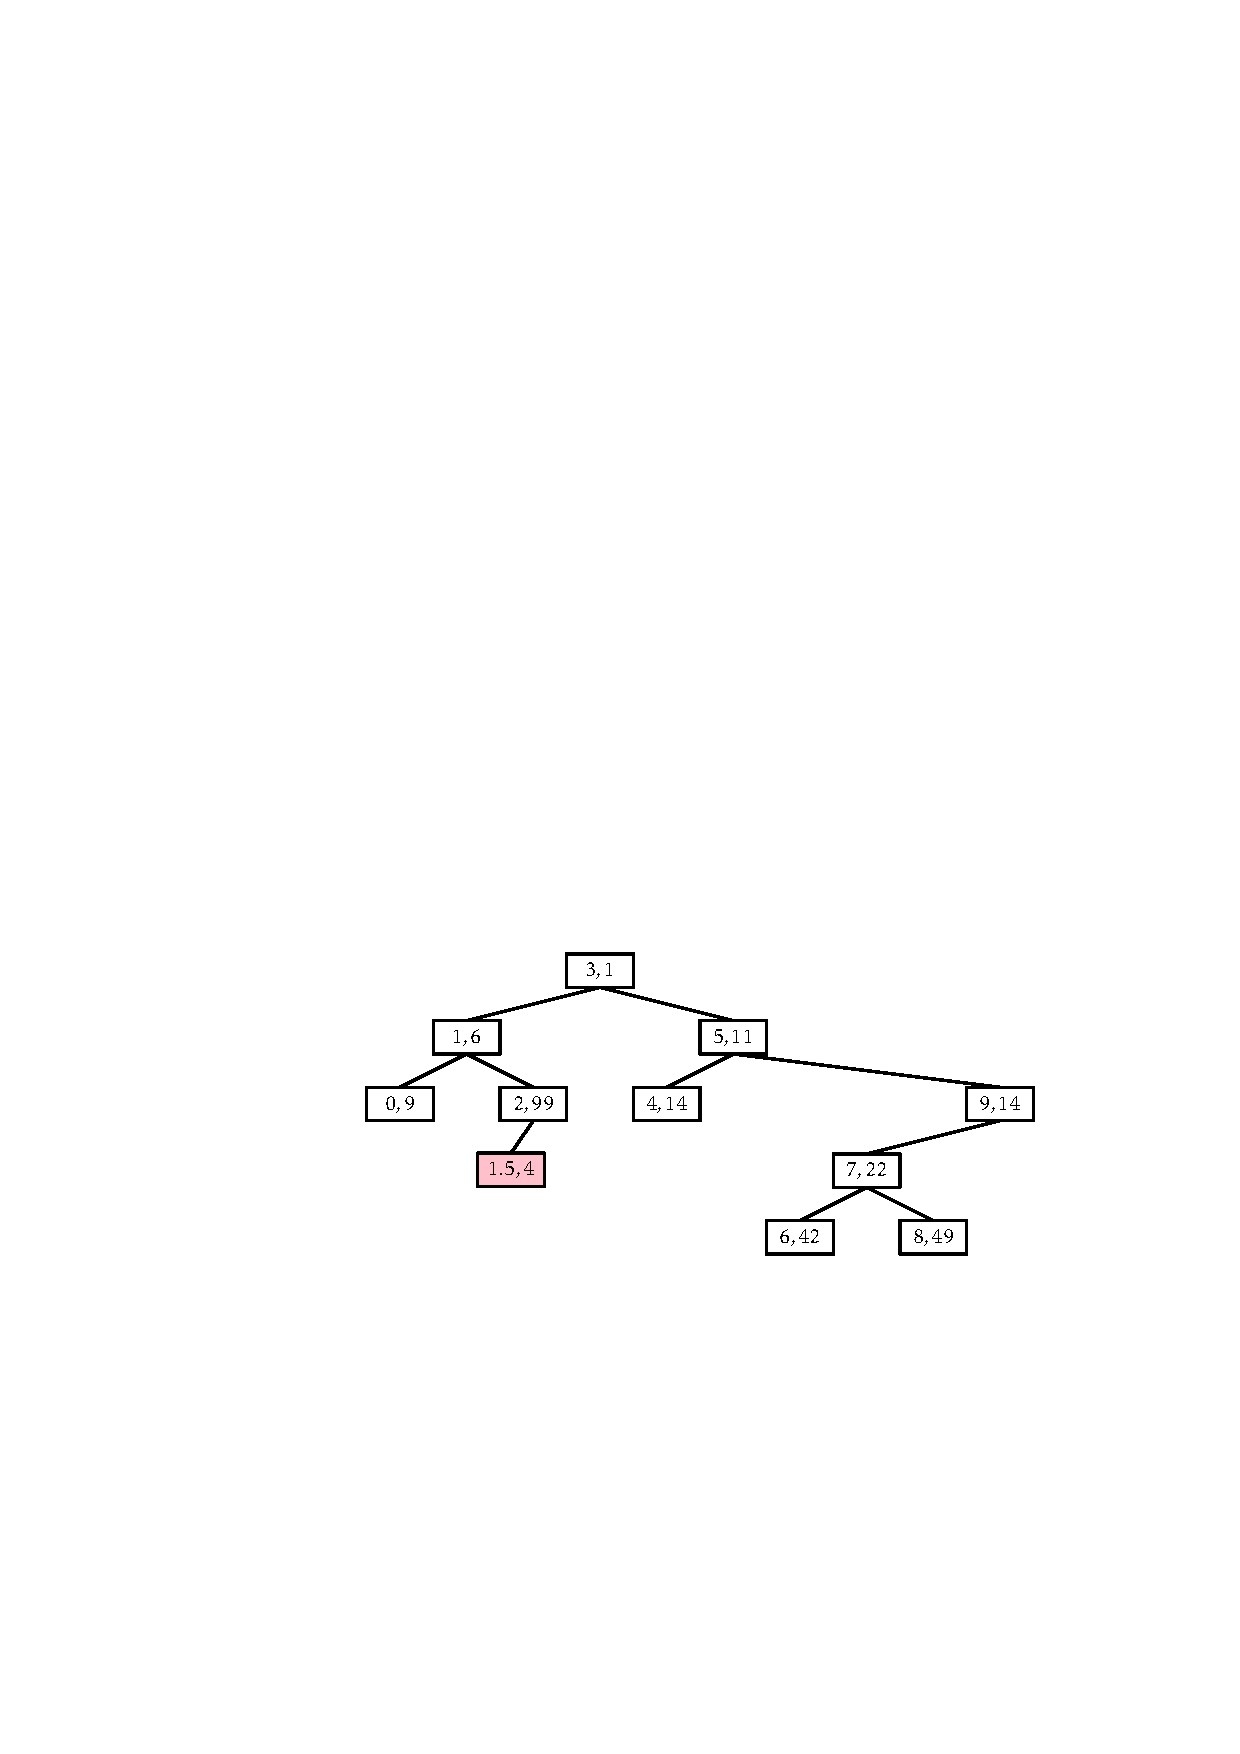
\includegraphics[width=\ScaleIfNeeded]{figs/treap-insert-a} \\
  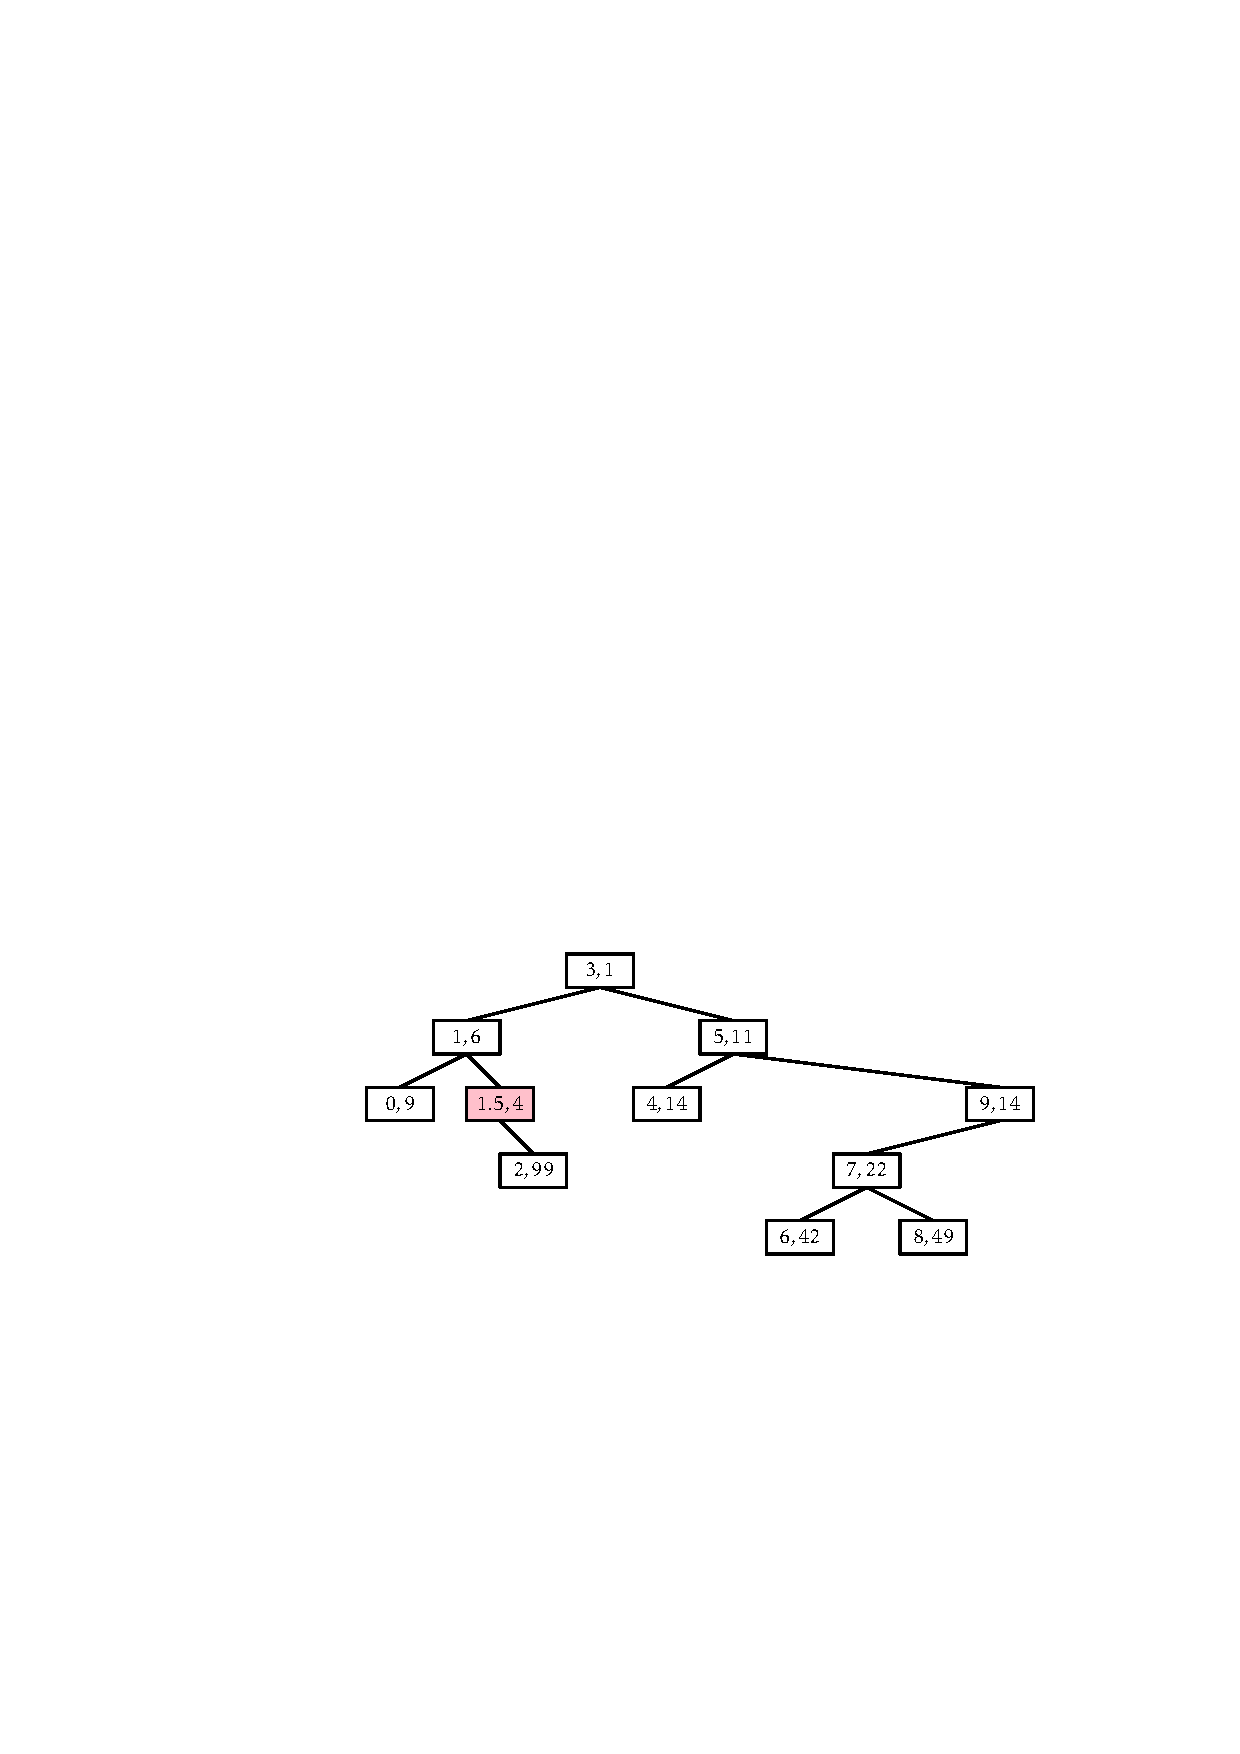
\includegraphics[width=\ScaleIfNeeded]{figs/treap-insert-b} \\
  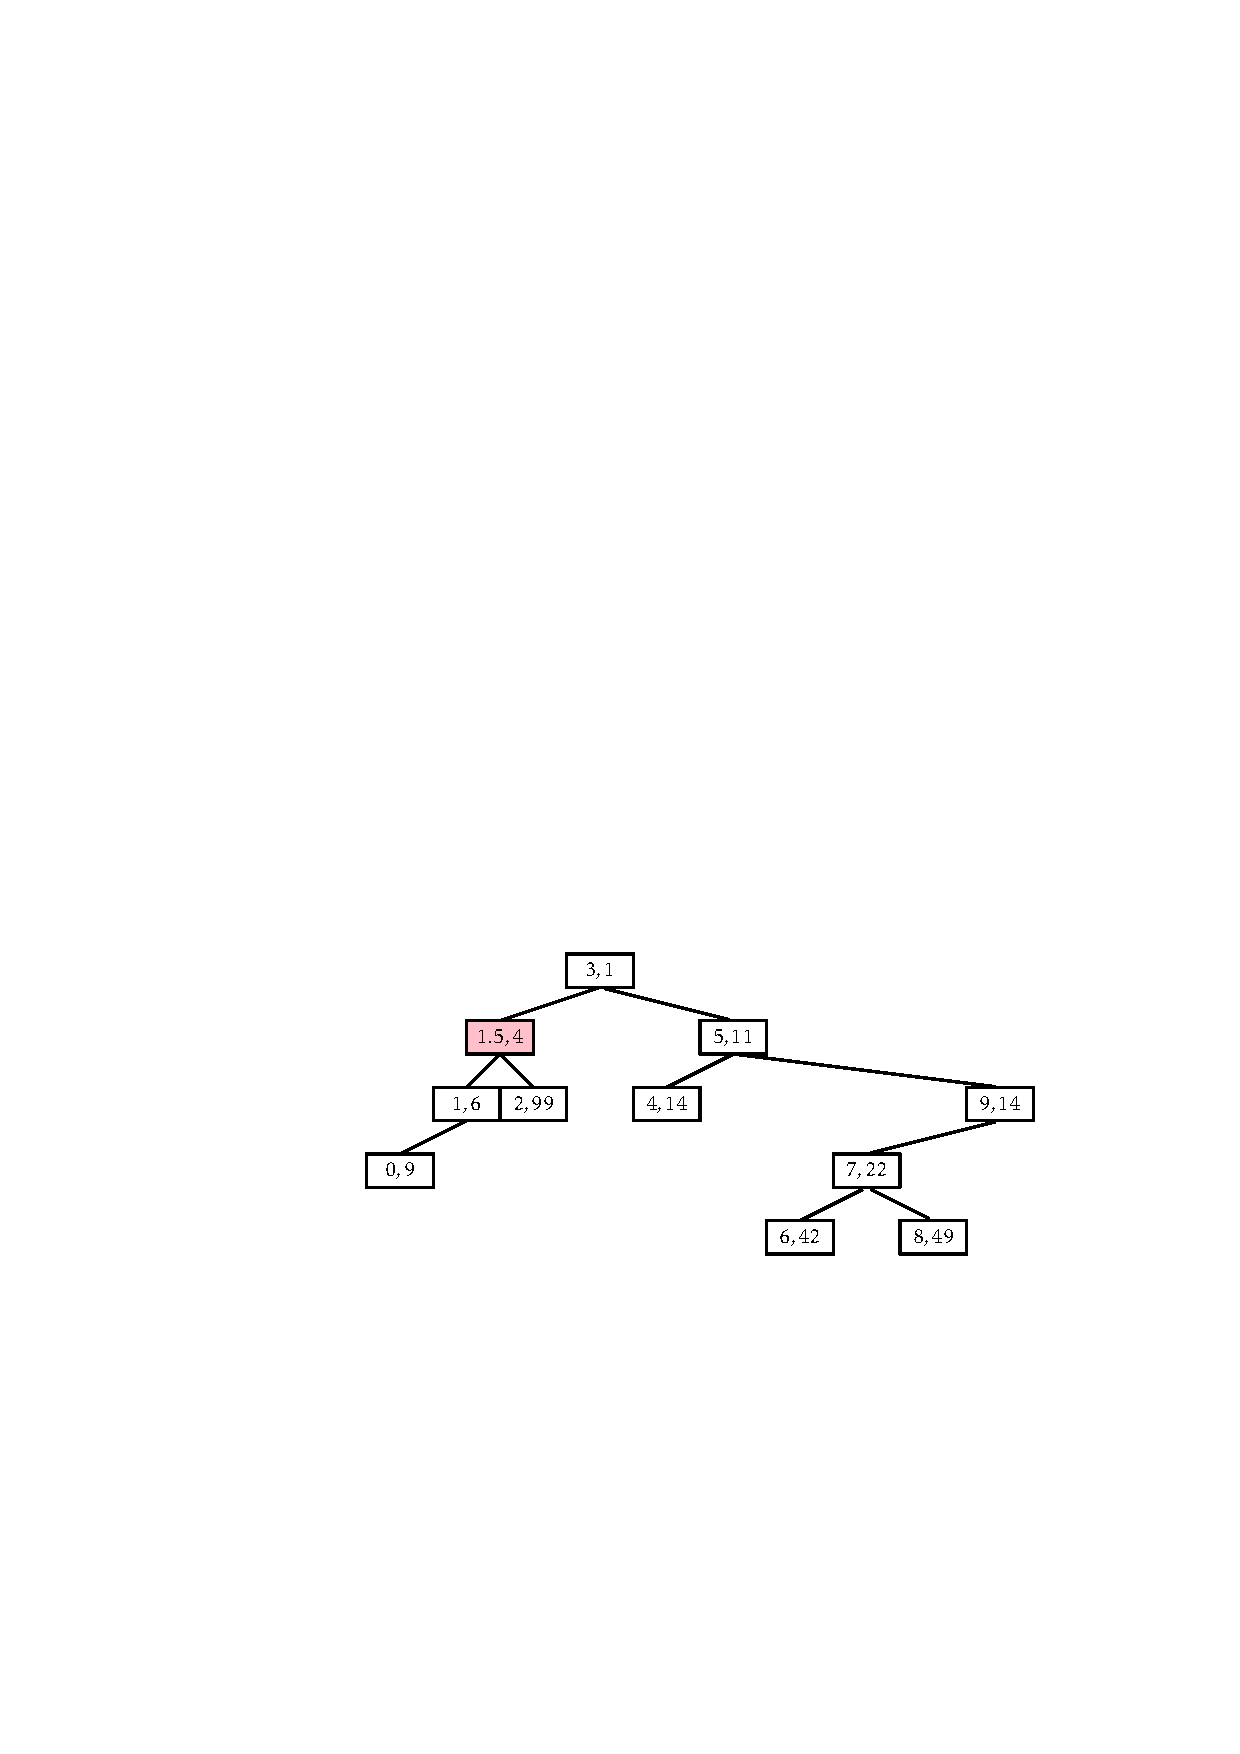
\includegraphics[width=\ScaleIfNeeded]{figs/treap-insert-c} \\
  \end{center}
  \caption[Adding to a Treap]{Adding the value 1.5 into the #Treap# from \figref{treap}.}
  \figlabel{treap-add}
\end{figure}

The running time of the #add(x)# operation is given by the time it
takes to follow the search path for #x# plus the number of rotations
performed to move the newly-added node, #u#, up to its correct location
in the #Treap#.  By \lemref{rbs-treap}, the expected length of the
search path is at most $2\ln #n#+O(1)$.  Furthermore, each rotation
decreases the depth of #u#.   This stops if #u# becomes the root, so
the expected number of rotations cannot exceed the expected length of
the search path.  Therefore, the expected running time of the #add(x)#
operation in a #Treap# is $O(\log #n#)$.  (\excref{treap-rotates}
asks you to show that the expected number of rotations performed during
an addition is actually only $O(1)$.)

The #remove(x)# operation in a #Treap# is the opposite of the #add(x)#
operation.  We search for the node, #u#, containing #x#, then perform
rotations to move #u# downwards until it becomes a leaf, and then we
splice #u# from the #Treap#.  Notice that, to move #u# downwards, we can
perform either a left or right rotation at #u#, which will replace #u#
with #u.right# or #u.left#, respectively.
The choice is made by the first of the following that apply:
\begin{enumerate}
\item If #u.left# and #u.right# are both #null#, then #u# is a leaf and no rotation is performed.
\item If #u.left# (or #u.right#) is #null#, then perform a right (or left, respectively) rotation at #u#.
\item If $#u.left.p# < #u.right.p#$ (or $#u.left.p# > #u.right.p#)$, then perform a right rotation (or left rotation, respectively) at #u#.
\end{enumerate}
These three rules ensure that the #Treap# doesn't become disconnected and that the heap property is restored once #u# is removed.
\codeimport{ods/Treap.remove(x).trickleDown(u)}
An example of the #remove(x)# operation is shown in \figref{treap-remove}.
\begin{figure}
  \begin{center}
  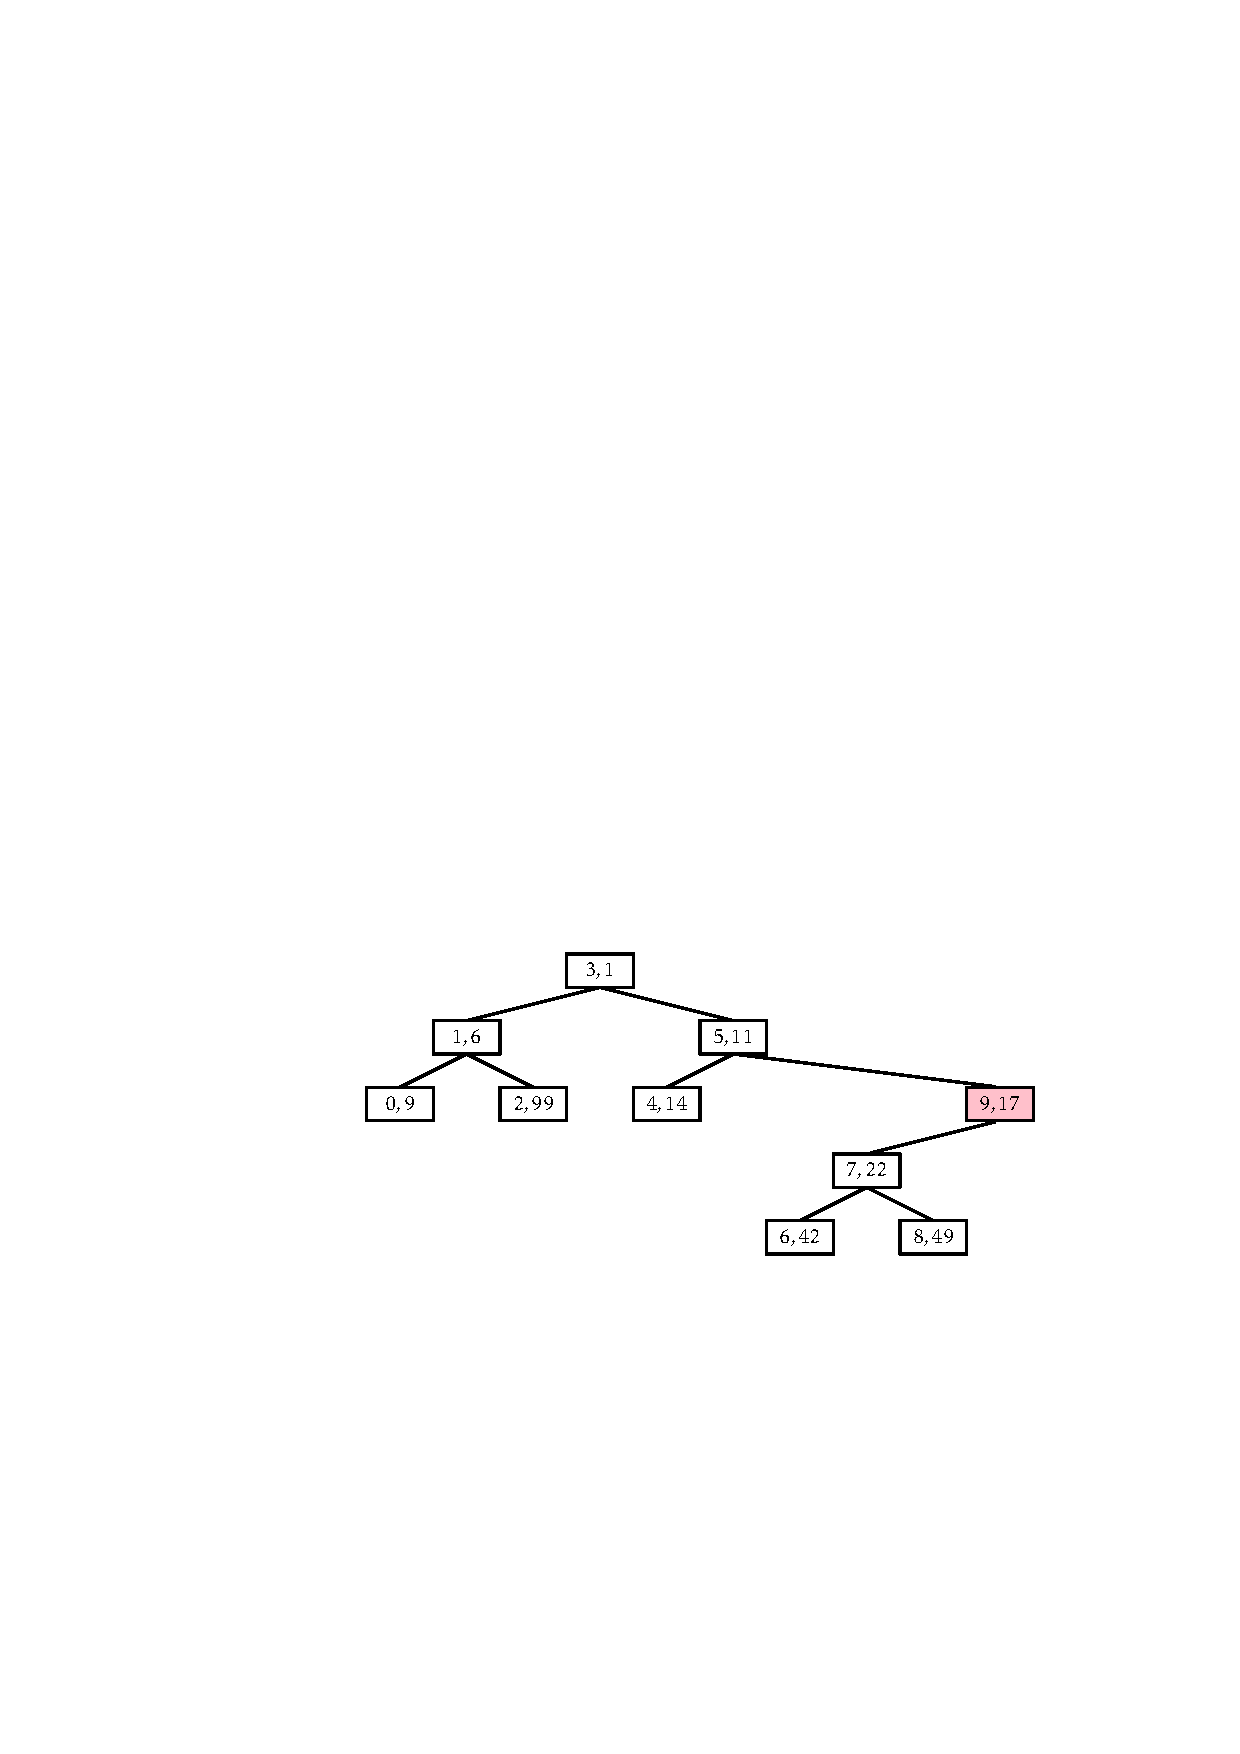
\includegraphics[height=\QuarterHeightScaleIfNeeded]{figs/treap-delete-a} \\
  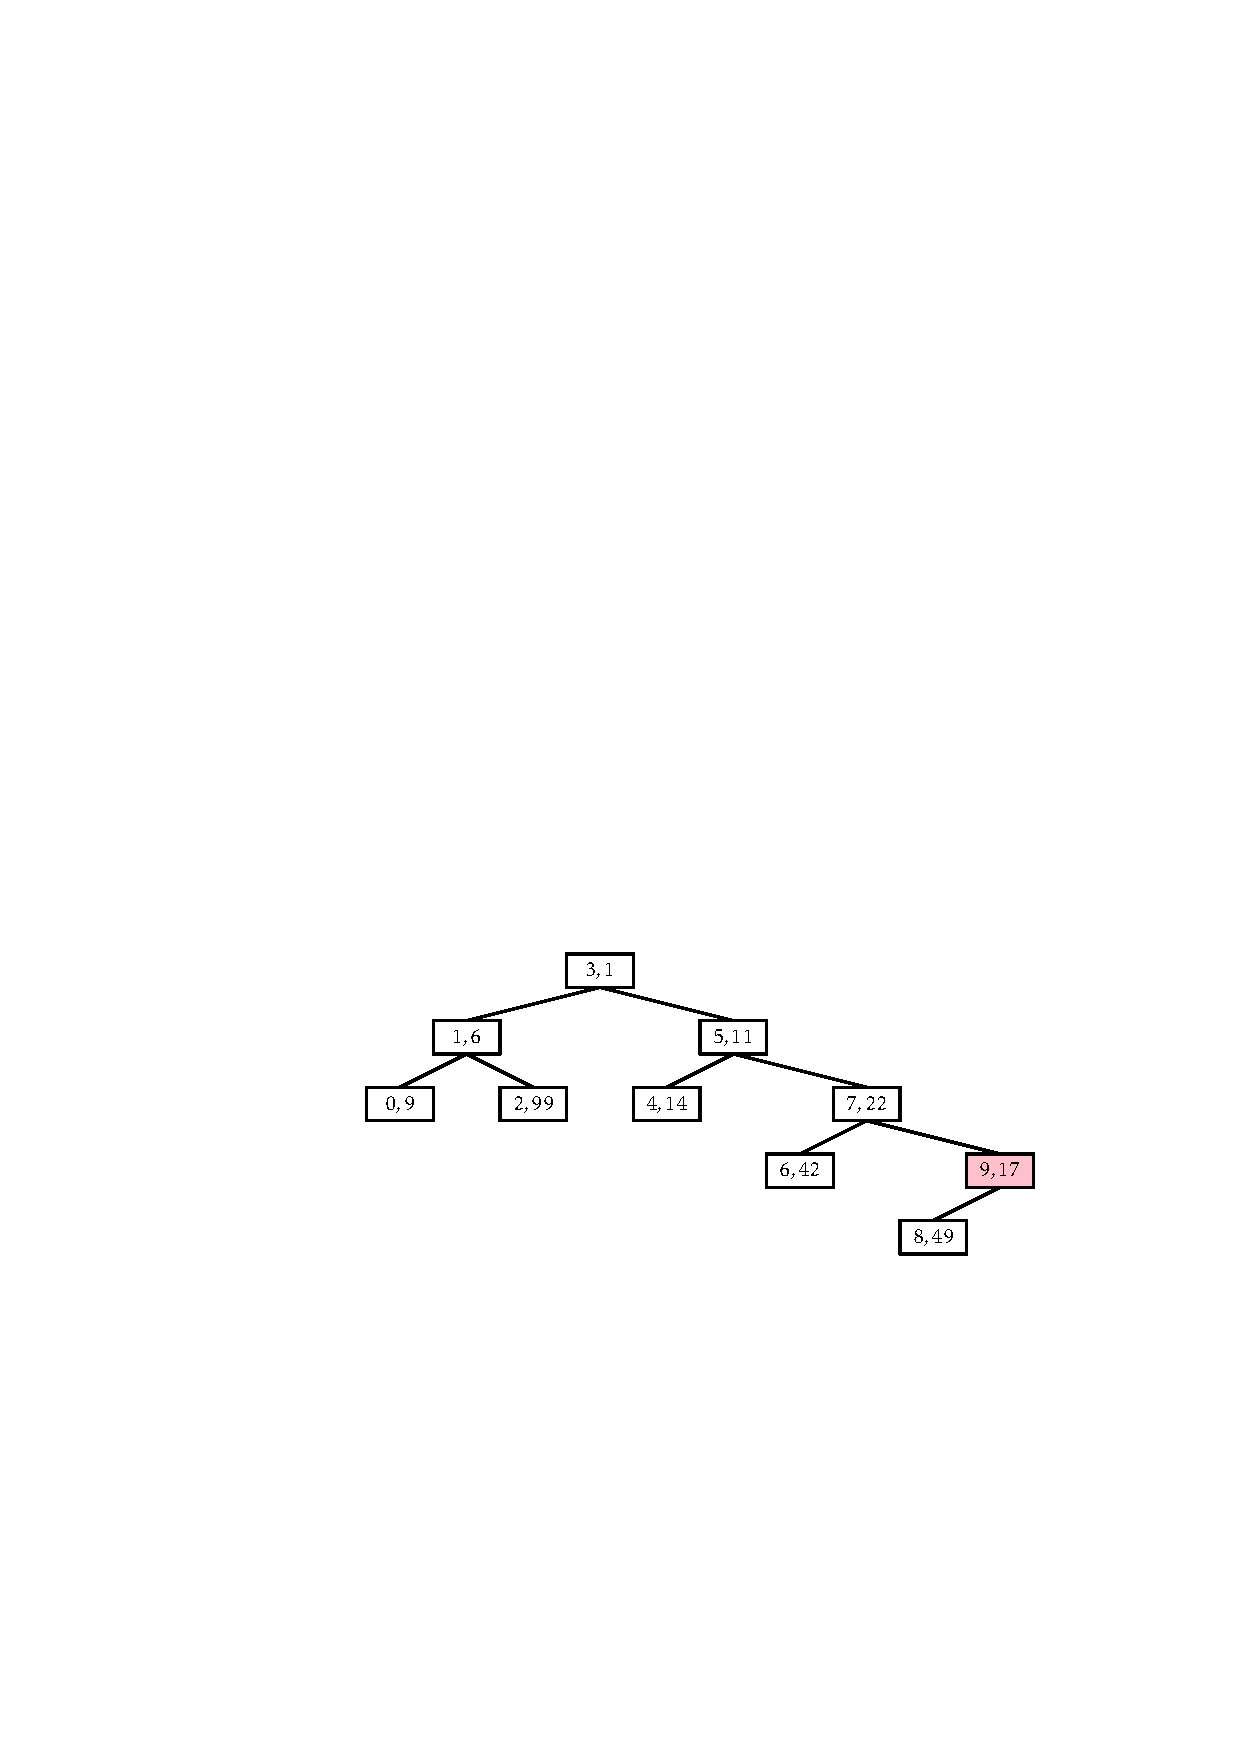
\includegraphics[height=\QuarterHeightScaleIfNeeded]{figs/treap-delete-b} \\
  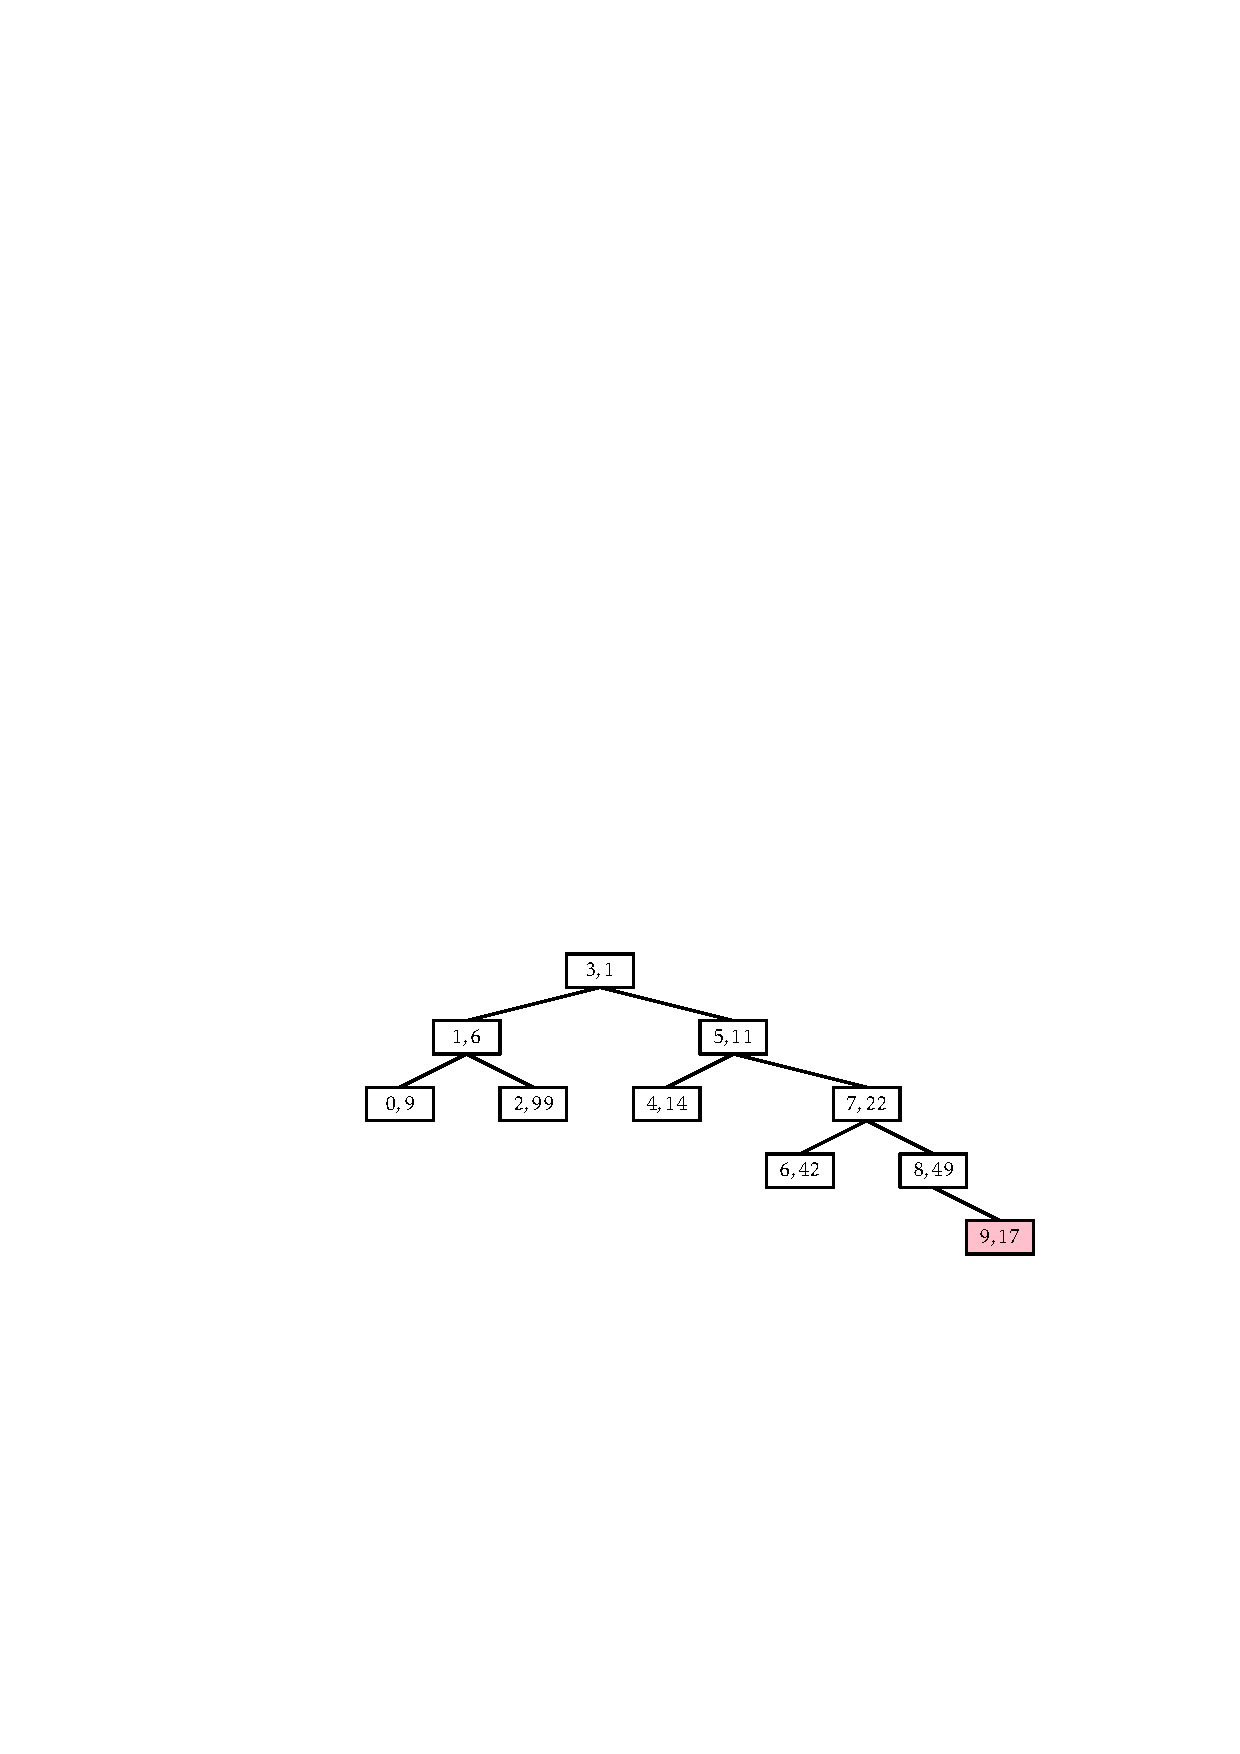
\includegraphics[height=\QuarterHeightScaleIfNeeded]{figs/treap-delete-c} \\
  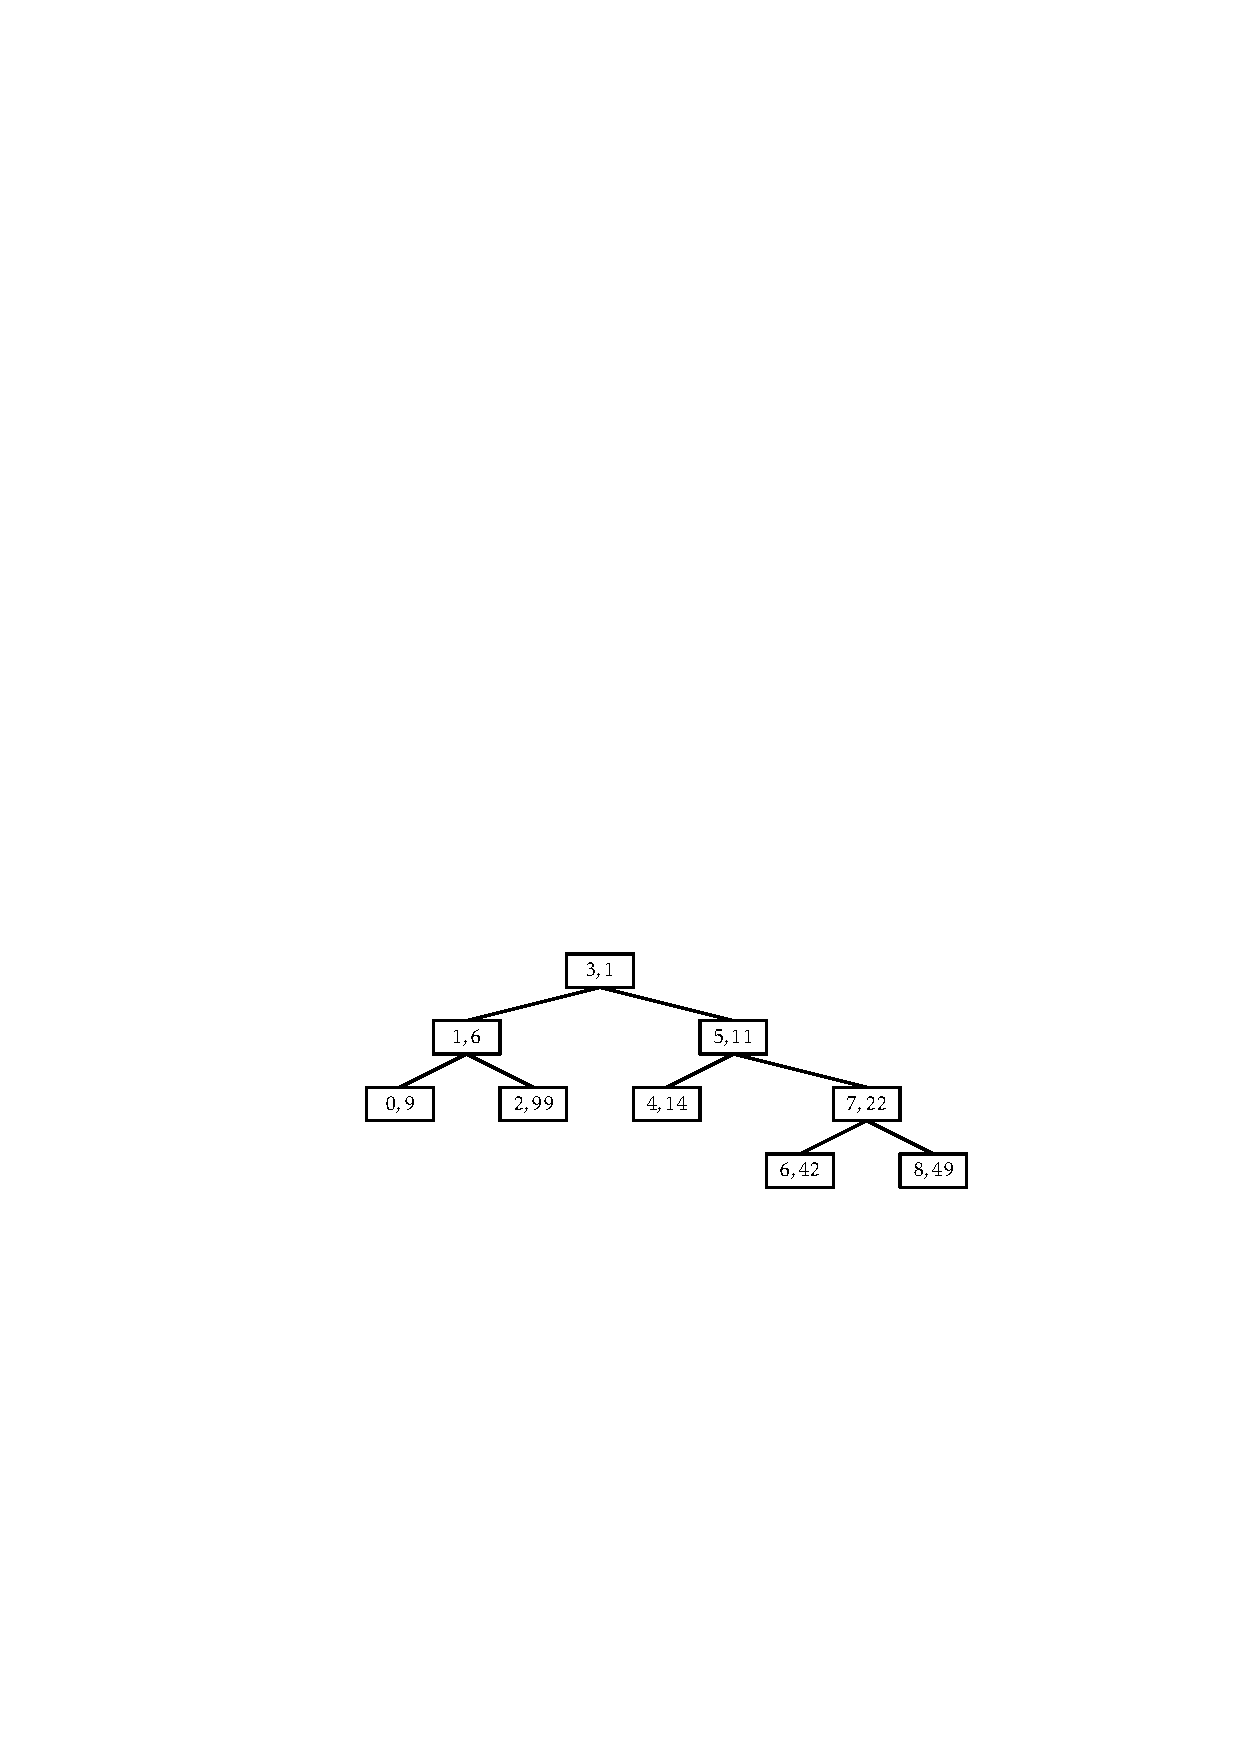
\includegraphics[height=\QuarterHeightScaleIfNeeded]{figs/treap-delete-d} 
  \end{center}
  \caption[Removing from a treap]{Removing the value 9 from the #Treap# in \figref{treap}.}
  \figlabel{treap-remove}
\end{figure}

The trick to analyze the running time of the #remove(x)# operation is
to notice that this operation reverses the #add(x)# operation.
In particular, if we were to reinsert #x#, using the same priority #u.p#,
then the #add(x)# operation would do exactly the same number of rotations
and would restore the #Treap# to exactly the same state it was in before
the #remove(x)# operation took place.  (Reading from bottom-to-top,
\figref{treap-remove} illustrates the addition of the value 9 into a
#Treap#.) This means that the expected running time of the #remove(x)#
on a #Treap# of size #n# is proportional to the expected running time
of the #add(x)# operation on a #Treap# of size $#n#-1$.  We conclude
that the expected running time of #remove(x)# is $O(\log #n#)$.

\subsection{Summary}

The following theorem summarizes the performance of the #Treap# data
structure:

\begin{thm}
A #Treap# implements the #SSet# interface. A #Treap# supports
the operations #add(x)#, #remove(x)#, and #find(x)# in $O(\log #n#)$
expected time per operation.
\end{thm}

It is worth comparing the #Treap# data structure to the #SkiplistSSet#
data structure.  Both implement the #SSet# operations in $O(\log #n#)$
expected time per operation.  In both data structures, #add(x)# and
#remove(x)# involve a search and then a constant number of pointer changes
(see \excref{treap-rotates} below).  Thus, for both these structures,
the expected length of the search path is the critical value in assessing
their performance.  In a #SkiplistSSet#, the expected length of a search
path is
\[
     2\log #n# + O(1) \enspace ,
\]
In a #Treap#, the expected length of a search path is 
\[
    2\ln #n# +O(1) \approx 1.386\log #n#  + O(1) \enspace .
\]
Thus, the search paths in a #Treap# are considerably shorter and this
translates into noticeably faster operations on #Treap#s than #Skiplist#s.
\excref{skiplist-opt} in \chapref{skiplists} shows how the
expected length of the search path in a #Skiplist# can be reduced to
\[
     e\ln #n# + O(1) \approx 1.884\log #n# + O(1) 
\]
by using biased coin tosses.  Even with this optimization, the expected
length of search paths in a #SkiplistSSet# is noticeably longer than in
a #Treap#.

\section{Discussion and Exercises}

Random binary search trees have been studied extensively.  Devroye
\cite{d88} gives a proof of \lemref{rbs} and related results. There are
much stronger results in the literature as well, the most impressive
of which is due to Reed \cite{r03}, who shows that the expected height
of a random binary search tree is
\[
  \alpha\ln n - \beta\ln\ln n + O(1)
\]
where $\alpha\approx4.31107$ is the unique solution on the
interval $[2,\infty)$ of the equation $\alpha\ln((2e/\alpha))=1$ and
$\beta=\frac{3}{2\ln(\alpha/2)}$ .  Furthermore, the variance of the
height is constant.

The name #Treap# was coined by Seidel and Aragon \cite{as96} who discussed
#Treap#s and some of their variants.  However, their basic structure was
studied much earlier by Vuillemin \cite{v80} who called them Cartesian
trees.

One possible space-optimization of the #Treap# data structure 
is the elimination of the explicit storage of the priority #p#
in each node. Instead, the priority of a node, #u#, is computed by
hashing #u#'s address in memory\javaonly{ (in 32-bit Java, this is equivalent
to hashing #u.hashCode()#)}.  Although a number of hash functions will
probably work well for this in practice, for the important parts of the
proof of \lemref{rbs} to remain valid, the hash function should be randomized
and have the \emph{min-wise independent property}:
\index{min-wise independence}%
For any distinct
values $x_1,\ldots,x_k$, each of the hash values $h(x_1),\ldots,h(x_k)$
should be distinct with high probability and, for each $i\in\{1,\ldots,k\}$,
\[
   \Pr\{h(x_i) = \min\{h(x_1),\ldots,h(x_k)\}\} \le c/k
\]
for some constant $c$.
One such class of hash functions that is easy to implement and fairly
fast is \emph{tabulation hashing} (\secref{tabulation}).
\index{tabulation hashing}%
\index{hashing!tabulation}%

Another #Treap# variant that doesn't store priorities at each node is
the randomized binary search tree
\index{randomized binary search tree}%
\index{binary search tree!randomized}%
of Mart\'\i nez and Roura \cite{mr98}.
In this variant, every node, #u#, stores the size, #u.size#, of the
subtree rooted at #u#.  Both the #add(x)# and #remove(x)# algorithms are
randomized. The algorithm for adding #x# to the subtree rooted at #u#
does the following:
\begin{enumerate}
   \item With probability $1/(#size(u)#+1)$, the value #x# is added
   the usual way, as a leaf, and rotations are then done to bring #x#
   up to the root of this subtree.
   \item Otherwise (with probability $1-1/(#size(u)#+1)$), the value #x#
   is recursively added into one of the two subtrees rooted at #u.left#
   or #u.right#, as appropriate.
\end{enumerate}
The first case corresponds to an #add(x)# operation in a #Treap# where
#x#'s node receives a random priority that is smaller than any of the
#size(u)# priorities in #u#'s subtree, and this case occurs with exactly
the same probability.

Removing a value #x# from a randomized binary search tree is similar
to the process of removing from a #Treap#.  We find the node, #u#,
that contains #x# and then perform rotations that repeatedly increase
the depth of #u# until it becomes a leaf, at which point we can splice
it from the tree.  The choice of whether to perform a left or right
rotation at each step is randomized.
\begin{enumerate}
  \item With probability #u.left.size/(u.size-1)#, we perform a right
  rotation at #u#, making #u.left# the root of the subtree that was
  formerly rooted at #u#.
  \item  With probability #u.right.size/(u.size-1)#, we perform a left
  rotation at #u#, making #u.right# the root of the subtree that was
  formerly rooted at #u#.
\end{enumerate}
Again, we can easily verify that these are exactly the same probabilities
that the removal algorithm in a #Treap# will perform a left or right
rotation of #u#.

Randomized binary search trees have the disadvantage, compared to treaps,
that when adding and removing elements they make many random choices, and
they must maintain the sizes of subtrees.  One advantage of randomized
binary search trees over treaps is that subtree sizes can serve another
useful purpose, namely to provide access by rank in $O(\log #n#)$ expected
time (see \excref{treap-get}).  In comparison, the random priorities
stored in treap nodes have no use other than keeping the treap balanced.

\begin{exc}
  Illustrate the addition of 4.5 (with priority 7) and then 7.5 (with
  priority 20) on the #Treap# in \figref{treap}.
\end{exc}

\begin{exc}
  Illustrate the removal of 5 and then 7 on the #Treap# in \figref{treap}.
\end{exc}

\begin{exc}
  Prove the assertion that there are $21,964,800$ sequences that generate
  the tree on the right hand side of \figref{rbs-lvc}.  (Hint: Give a
  recursive formula for the number of sequences that generate a complete
  binary tree of height $h$ and evaluate this formula for $h=3$.)
\end{exc}

\begin{exc}
  Design and implement the #permute(a)# method that takes as input an
  array, #a#, that contains #n# distinct values and randomly permutes #a#.
  The method should run in $O(#n#)$ time and you should prove that each
  of the $#n#!$ possible permutations of #a# is equally probable. 
\end{exc}

\begin{exc}\exclabel{treap-rotates}
  Use both parts of \lemref{rbs-treap} to prove that the expected number
  of rotations performed by an #add(x)# operation (and hence also a
  #remove(x)# operation) is $O(1)$.
\end{exc}

\begin{exc}
  Modify the #Treap# implementation given here so that it does not
  explicitly store priorities.  Instead, it should simulate them by
  hashing the #hashCode()# of each node.
\end{exc}

\begin{exc}
  Suppose that a binary search tree stores, at each node, #u#, the height,
  #u.height#, of the subtree rooted at #u#, and the size, #u.size# of
  the subtree rooted at #u#. 
  \begin{enumerate}
    \item Show how, if we perform a left or right
      rotation at #u#, then these two quantities can be updated, in
      constant time, for all nodes affected by the rotation.
    \item Explain why the same result is not possible if we try to
      also store the depth, #u.depth#, of each node #u#.
  \end{enumerate}
\end{exc}

\begin{exc}
  Design and implement an algorithm that constructs a #Treap# from a
  sorted array, #a#, of #n# elements.  This method should run in $O(#n#)$
  worst-case time and should construct a #Treap# that is indistinguishable
  from one in which the elements of #a# were added one at a time using
  the #add(x)# method.
\end{exc}


\begin{exc}
  \index{finger}%
  \index{finger search!in a treap}%
  This exercise works out the details of how one can efficiently search
  a #Treap# given a pointer that is close to the node we are searching for.
  \begin{enumerate}
    \item Design and implement a #Treap# implementation in which each
      node keeps track of the minimum and maximum values in its subtree.
    \item Using this extra information, add a #fingerFind(x,u)# method
      that executes the #find(x)# operation with the help of a pointer
      to the node #u# (which is hopefully not far from the node that
      contains #x#).  This operation should start at #u# and walk upwards
      until it reaches a node #w# such that $#w.min#\le #x#\le #w.max#$.
      From that point onwards, it should perform a standard search
      for #x# starting from #w#.  (One can show that #fingerFind(x,u)#
      takes $O(1+\log r)$ time, where $r$ is the number of elements in
      the treap whose value is between #x# and #u.x#.)
    \item Extend your implementation into a version of a treap that
      starts all its #find(x)# operations from the node most recently
      found by #find(x)#.
  \end{enumerate}
\end{exc}

\begin{exc}\exclabel{treap-get}
  Design and implement a version of a #Treap# that includes a #get(i)#
  operation that returns the key with rank #i# in the #Treap#.  (Hint:
  Have each node, #u#, keep track of the size of the subtree rooted
  at #u#.)
\end{exc}

\begin{exc}
  \index{TreapList@#TreapList#}%
  Implement a #TreapList#, an implementation of the #List# interface
  as a treap.  Each node in the treap should store a list item, and an
  in-order traversal of the treap finds the items in the same order that
  they occur in the list.  All the #List# operations #get(i)#, #set(i,x)#,
  #add(i,x)# and #remove(i)# should run in $O(\log #n#)$ expected time.
\end{exc}



\begin{exc}\exclabel{treap-split}
  Design and implement a version of a #Treap# that supports the #split(x)#
  operation.  This operation removes all values from the #Treap# that
  are greater than #x# and returns a second #Treap# that contains all
  the removed values.

  \noindent Example: the code #t2 = t.split(x)# removes from #t# all values
  greater than #x# and returns a new #Treap# #t2# containing all
  these values. The #split(x)# operation should run in $O(\log #n#)$
  expected time.

  \noindent Warning: For this modification to work properly and still allow the
  #size()# method to run in constant time, it is necessary to implement
  the modifications in \excref{treap-get}.
\end{exc}

\begin{exc}\exclabel{treap-join}
  Design and implement a version of a #Treap# that supports the
  #absorb(t2)# operation, which can be thought of as the inverse of
  the #split(x)# operation.  This operation removes all values from the
  #Treap# #t2# and adds them to the receiver.  This operation presupposes
  that the smallest value in #t2# is greater than the largest value in
  the receiver.  The #absorb(t2)# operation should run in $O(\log #n#)$
  expected time.
\end{exc}

\begin{exc}
  Implement Martinez's randomized binary search trees, as discussed in
  this section.  Compare the performance of your implementation with
  that of the #Treap# implementation.
\end{exc}

